% Created 2017-02-09 Thu 13:14
\documentclass[11pt]{article}
\usepackage[utf8]{inputenc}
\usepackage[T1]{fontenc}
\usepackage{fixltx2e}
\usepackage{graphicx}
\usepackage{longtable}
\usepackage{float}
\usepackage{wrapfig}
\usepackage{rotating}
\usepackage[normalem]{ulem}
\usepackage{amsmath}
\usepackage{textcomp}
\usepackage{marvosym}
\usepackage{wasysym}
\usepackage{amssymb}
\usepackage{hyperref}
\tolerance=1000
\author{David A. Ventimiglia\thanks{dventimi@gmail.com}}
\date{\textit{<2017-02-08>}}
\title{Advanced Lane Lines}
\hypersetup{
  pdfkeywords={},
  pdfsubject={},
  pdfcreator={<a href="http://www.gnu.org/software/emacs/">Emacs</a> 24.5.1 (<a href="http://orgmode.org">Org</a> mode 8.2.10)}}
\begin{document}

\maketitle

\index{Machine-Learning!Self-Driving Cars}
\index{Udacity!Self-Driving Car Nano-Degree Program}

\section*{Introduction}
\label{sec-1}

\section*{Methods}
\label{sec-2}

The goals / steps of this project are the following:

\begin{itemize}
\item Compute the camera calibration matrix and distortion coefficients
given a set of chessboard images.
\item Apply a distortion correction to raw images.
\item Use color transforms, gradients, etc., to create a thresholded
binary image.
\item Apply a perspective transform to rectify binary image ("birds-eye
view").
\item Detect lane pixels and fit to find the lane boundary.
\item Determine the curvature of the lane and vehicle position with
respect to center.
\item Warp the detected lane boundaries back onto the original image.
\item Output visual display of the lane boundaries and numerical
estimation of lane curvature and vehicle position.
\end{itemize}

\subsection*{Setup}
\label{sec-2-1}

The initial setup includes creating the \href{https://www.python.org/}{Python} environment with
the packages that the project needs and uses.

\begin{description}
\item[{\href{http://matplotlib.org/}{matplotlib}}] plotting and image processing tools
\item[{\href{http://www.numpy.org/}{NumPy}}] foundational scientific computing library
\item[{\href{http://zulko.github.io/moviepy/}{MoviePy}}] video processing tools
\item[{\href{http://opencv.org/}{OpenCV}}] computer vision library
\end{description}

The \href{https://github.com/}{GitHub} \href{https://github.com/dventimi/CarND-Advanced-Lane-Lines}{repository} for this project contains an \href{environment.yml}{environment.yml}
file that can be used to create and activate a \href{https://conda.io/docs/}{Conda} environment
with these commands.

\begin{verbatim}
conda env create --file environment.yml --name CarND-Advanced-Lane-Lines
source activate CarND-Advanced-Lane-Lines
\end{verbatim}

Once activated this environment is used to launch Python in
whatever way one likes, such as a \href{https://www.python.org/shell/}{Python shell}, a \href{https://ipython.org/}{IPython shell},
or a \href{http://jupyter.org/}{jupyter notebook}.  Having done that, the usual first step is
to import the packages that are used.  

\begin{verbatim}
from collections import deque
from itertools import groupby, islice, zip_longest, cycle, filterfalse
from moviepy.editor import VideoFileClip
import cProfile
import cv2
import glob
import matplotlib
import matplotlib.image as mpimg
import matplotlib.pyplot as plt
import numpy as np
import pdb
\end{verbatim}

Besides the third-party packages listed above, the project also
makes use of these standard-library library packages.

\begin{description}
\item[{deque}] \href{https://en.wikipedia.org/wiki/Circular_buffer}{ring buffers} for moving averages
\item[{itertools}] handy for \href{http://davidaventimiglia.com/python_generators.html}{Python generators}
\item[{cProfile}] run-time \href{https://docs.python.org/2/library/profile.html}{optimization}
\item[{pdb}] Python \href{https://docs.python.org/3/library/pdb.html}{debugger}
\end{description}


\subsection*{Processing Pipeline}
\label{sec-2-2}

In order to detect lane lines in a video of a car driving on a
road, and then generate an annotated video with the detected lane
overlaid, we need an image processor that performs these two
tasks--detection and annotation--on every frame of the video.
That image processor encompasses a "processing pipeline."  

The pipeline depends on these preliminary tasks.

\begin{enumerate}
\item Camera Calibration
\item Perspective Measurement
\end{enumerate}

Then, the pipeline applies these stages.

\begin{enumerate}
\item Distortion Correction
\item Gradient and Color Thresholds
\item Perspective Transform
\item Lane-line Detection
\end{enumerate}

Let us examine these preliminary tasks and pipeline stages in
greater detail.

\subsubsection*{Camera Calibration}
\label{sec-2-2-1}

\href{http://docs.opencv.org/2.4/modules/calib3d/doc/camera_calibration_and_3d_reconstruction.html}{Camera calibration} measures the distortion inherent in cameras
that utilize lenses so that the images taken with the camera can
be corrected by removing the distortion.  A standard way to do
this is to measure the distortion the camera imposes on standard
images of known geometry.  Checkerboard patterns are useful for
this tasks because of their high contrast, known geometry, and
regular pattern.

The \texttt{measure\_distortion} function takes a Python \href{https://docs.python.org/2/library/stdtypes.html#sequence-types-str-unicode-list-tuple-bytearray-buffer-xrange}{sequence} of
checkerboard image filenames taken at different distances,
center-offsets, and orientations and applies the OpenCV
functions \href{http://docs.opencv.org/2.4/modules/calib3d/doc/camera_calibration_and_3d_reconstruction.html#findchessboardcorners}{\texttt{findChessboardCorners}} and \href{http://docs.opencv.org/2.4/modules/calib3d/doc/camera_calibration_and_3d_reconstruction.html#drawchessboardcorners}{\texttt{drawChessboardCorners}} to
identify corners in the images and highlight the corners.  Then,
the \href{http://docs.opencv.org/2.4/modules/calib3d/doc/camera_calibration_and_3d_reconstruction.html#calibratecamera}{\texttt{calibrateCamera}} function measures the distortion.  This
function returns the distortion parameters and matrix, along
with a sequence of tuples with the original filenames and the
annotated images.

\begin{verbatim}
def measure_distortion(calibration_files):
    files = calibration_files
    objp = np.zeros((9*6,3), np.float32)
    objp[:,:2] = np.mgrid[0:9,0:6].T.reshape(-1,2)
    stage1 = map(lambda x: (x,), cycle(files))
    stage2 = map(lambda x: x + (mpimg.imread(x[0]),), stage1)
    stage3 = map(lambda x: x + (cv2.findChessboardCorners(cv2.cvtColor(x[1], cv2.COLOR_RGB2GRAY), (9,6)),), stage2)
    stage4 = map(lambda x: x + (cv2.drawChessboardCorners(np.copy(x[1]), (9,6), *(x[2][::-1])),), stage3)
    filenames,images,corners,annotated_images = zip(*filter(lambda x: x[2][0], islice(stage4, len(files))))
    _,imgpoints = zip(*corners)
    objpoints = [objp for i in range(len(imgpoints))]
    ret, mtx, dist, rvecs, tvecs = cv2.calibrateCamera(objpoints, imgpoints, list(islice(stage2,1))[0][1].shape[:2:][::-1], None, None)
    return mtx, dist, zip(filenames, annotated_images)
\end{verbatim}

This function is used in subsequent distortion corrections.

\subsubsection*{Distortion Correction}
\label{sec-2-2-2}

The \texttt{get\_undistorter} function takes a sequence of calibration
checkerboard image filenames, applies the \texttt{measure\_distortion}
function, and returns a new function.  The new function function
uses the OpenCV \href{http://docs.opencv.org/2.4/modules/imgproc/doc/geometric_transformations.html#void\%20undistort(InputArray\%20src,\%20OutputArray\%20dst,\%20InputArray\%20cameraMatrix,\%20InputArray\%20distCoeffs,\%20InputArray\%20newCameraMatrix)}{\texttt{undistort}} function to remove distortion from
images taken with the same camera.

\begin{verbatim}
def get_undistorter(calibration_files):
    mtx,dist,annotated_images = measure_distortion(calibration_files)
    return lambda x: cv2.undistort(x, mtx, dist, None, mtx), annotated_images
\end{verbatim}

In the example shown below, we get an "image undistorter"
function for a set of calibration images.

\begin{verbatim}
undistort,annotated_images = get_undistorter(glob.glob("camera_cal/*.jpg"))
fig = plt.figure()
grid = ImageGrid(fig, 111, nrows_ncols=(4,4), axes_pad=0.0)

for p in zip(annotated_images, grid):
    p[1].imshow(p[0][1])

fig.savefig("output_images/annotated_calibration_images.jpg")
\end{verbatim}

The annotated calibration images are shown in the figure below.

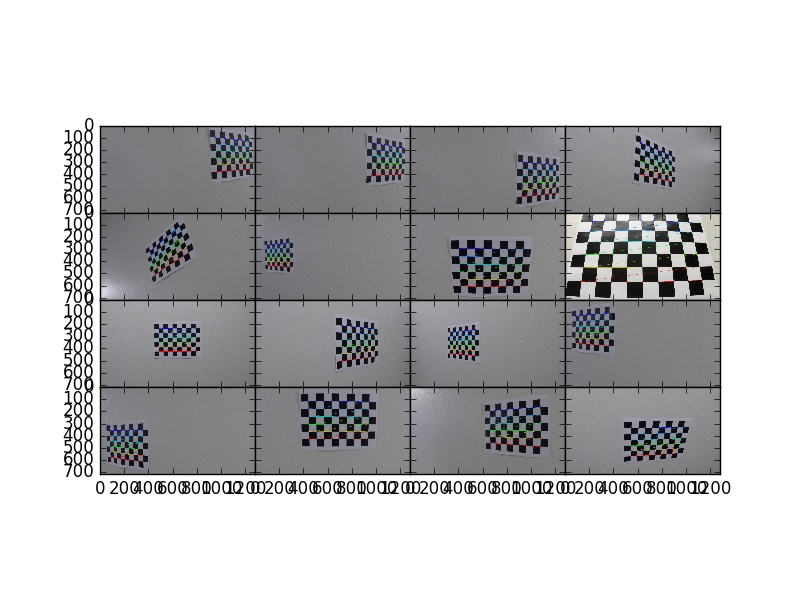
\includegraphics[width=.9\linewidth]{output_images/annotated_calibration_images.jpg}

We show the effects of applying the image undistorter to a
sequence of 6 road images taken with this same camera.  These 6
images are a test sequence that will reappear many times through
the remainder of this discussion as other image processing steps
are taken up.  

The \texttt{visualize} function helps us view a gallery of test images
in "ganged up" layout, and this is helpful as we develop the
processing pipeline stages.

\begin{verbatim}
def visualize(filename, a):
    fig, axes = plt.subplots(2,3,figsize=(24,12),subplot_kw={'xticks':[],'yticks':[]})
    fig.subplots_adjust(hspace=0.03, wspace=0.05)
    for p in zip(sum(axes.tolist(),[]), a):
	p[0].imshow(p[1],cmap='gray')
    plt.tight_layout()
    fig.savefig(filename)
    plt.close()
\end{verbatim}

The 6 test images that we use repeatedly are shown in the figure
below, without any image processing at all.

\begin{verbatim}
visualize("output_images/test_images.jpg",
	  (mpimg.imread(f) for f in cycle(glob.glob("test_images/test*.jpg"))))
\end{verbatim}

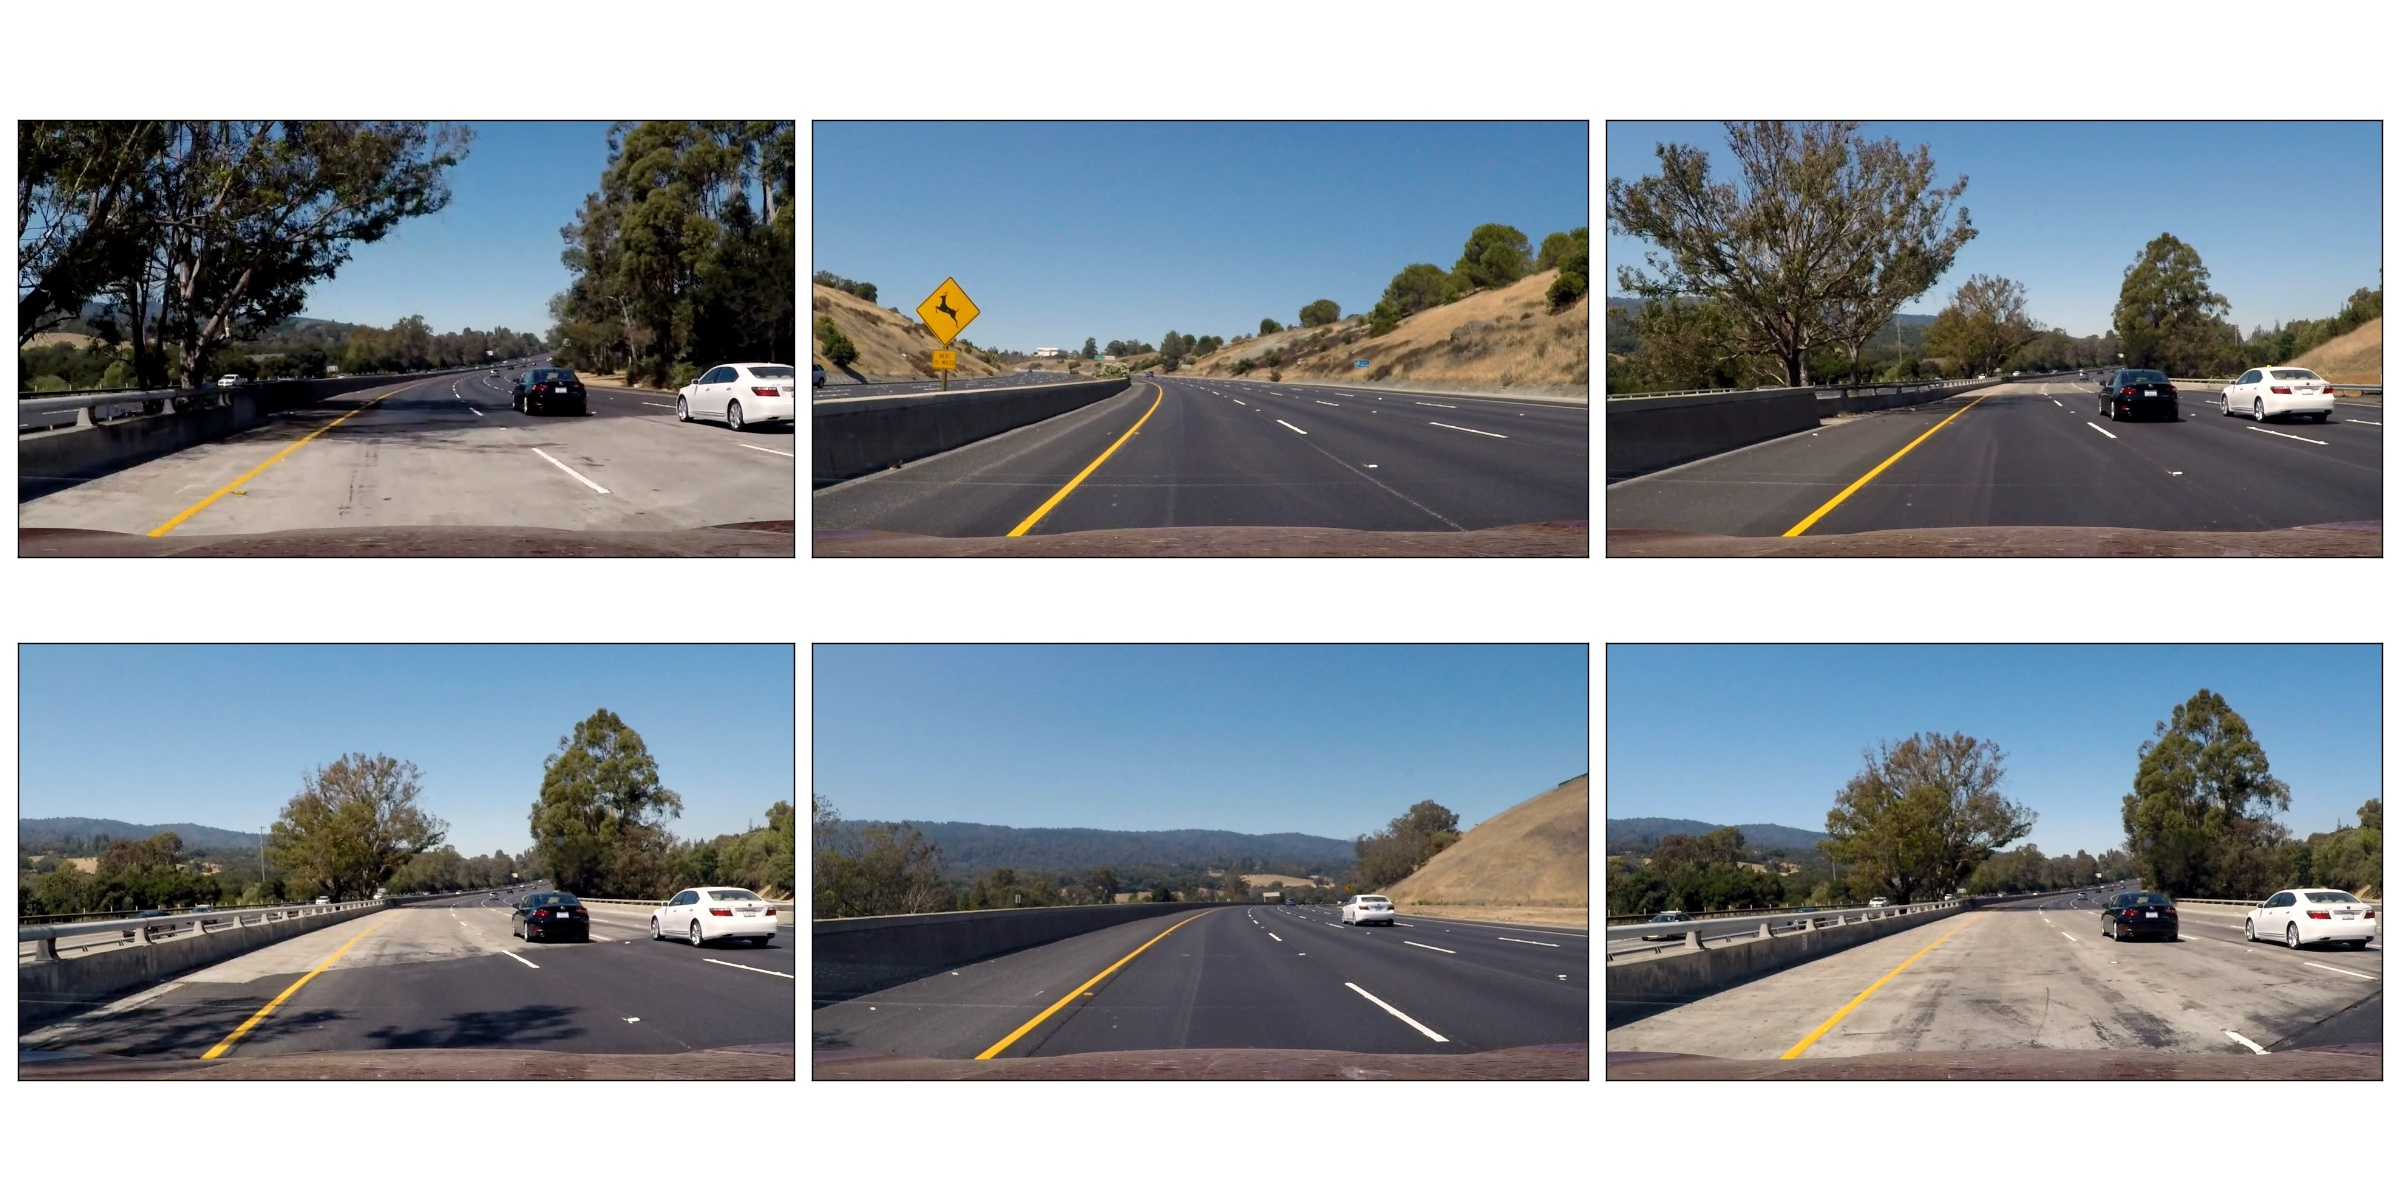
\includegraphics[width=.9\linewidth]{output_images/test_images.jpg}

These test images are shown again, only this time the image
undistorter that we acquired above now is used to remove
distortion introduced by the camera.  The effect is subtle and
difficult to notice, but close inspection shows that at least a
small amount of radial distortion is removed by this process.  

\begin{verbatim}
visualize("output_images/undistorted_test_images.jpg",
	  (undistort(mpimg.imread(f)) for f in cycle(glob.glob("test_images/test*.jpg"))))
\end{verbatim}

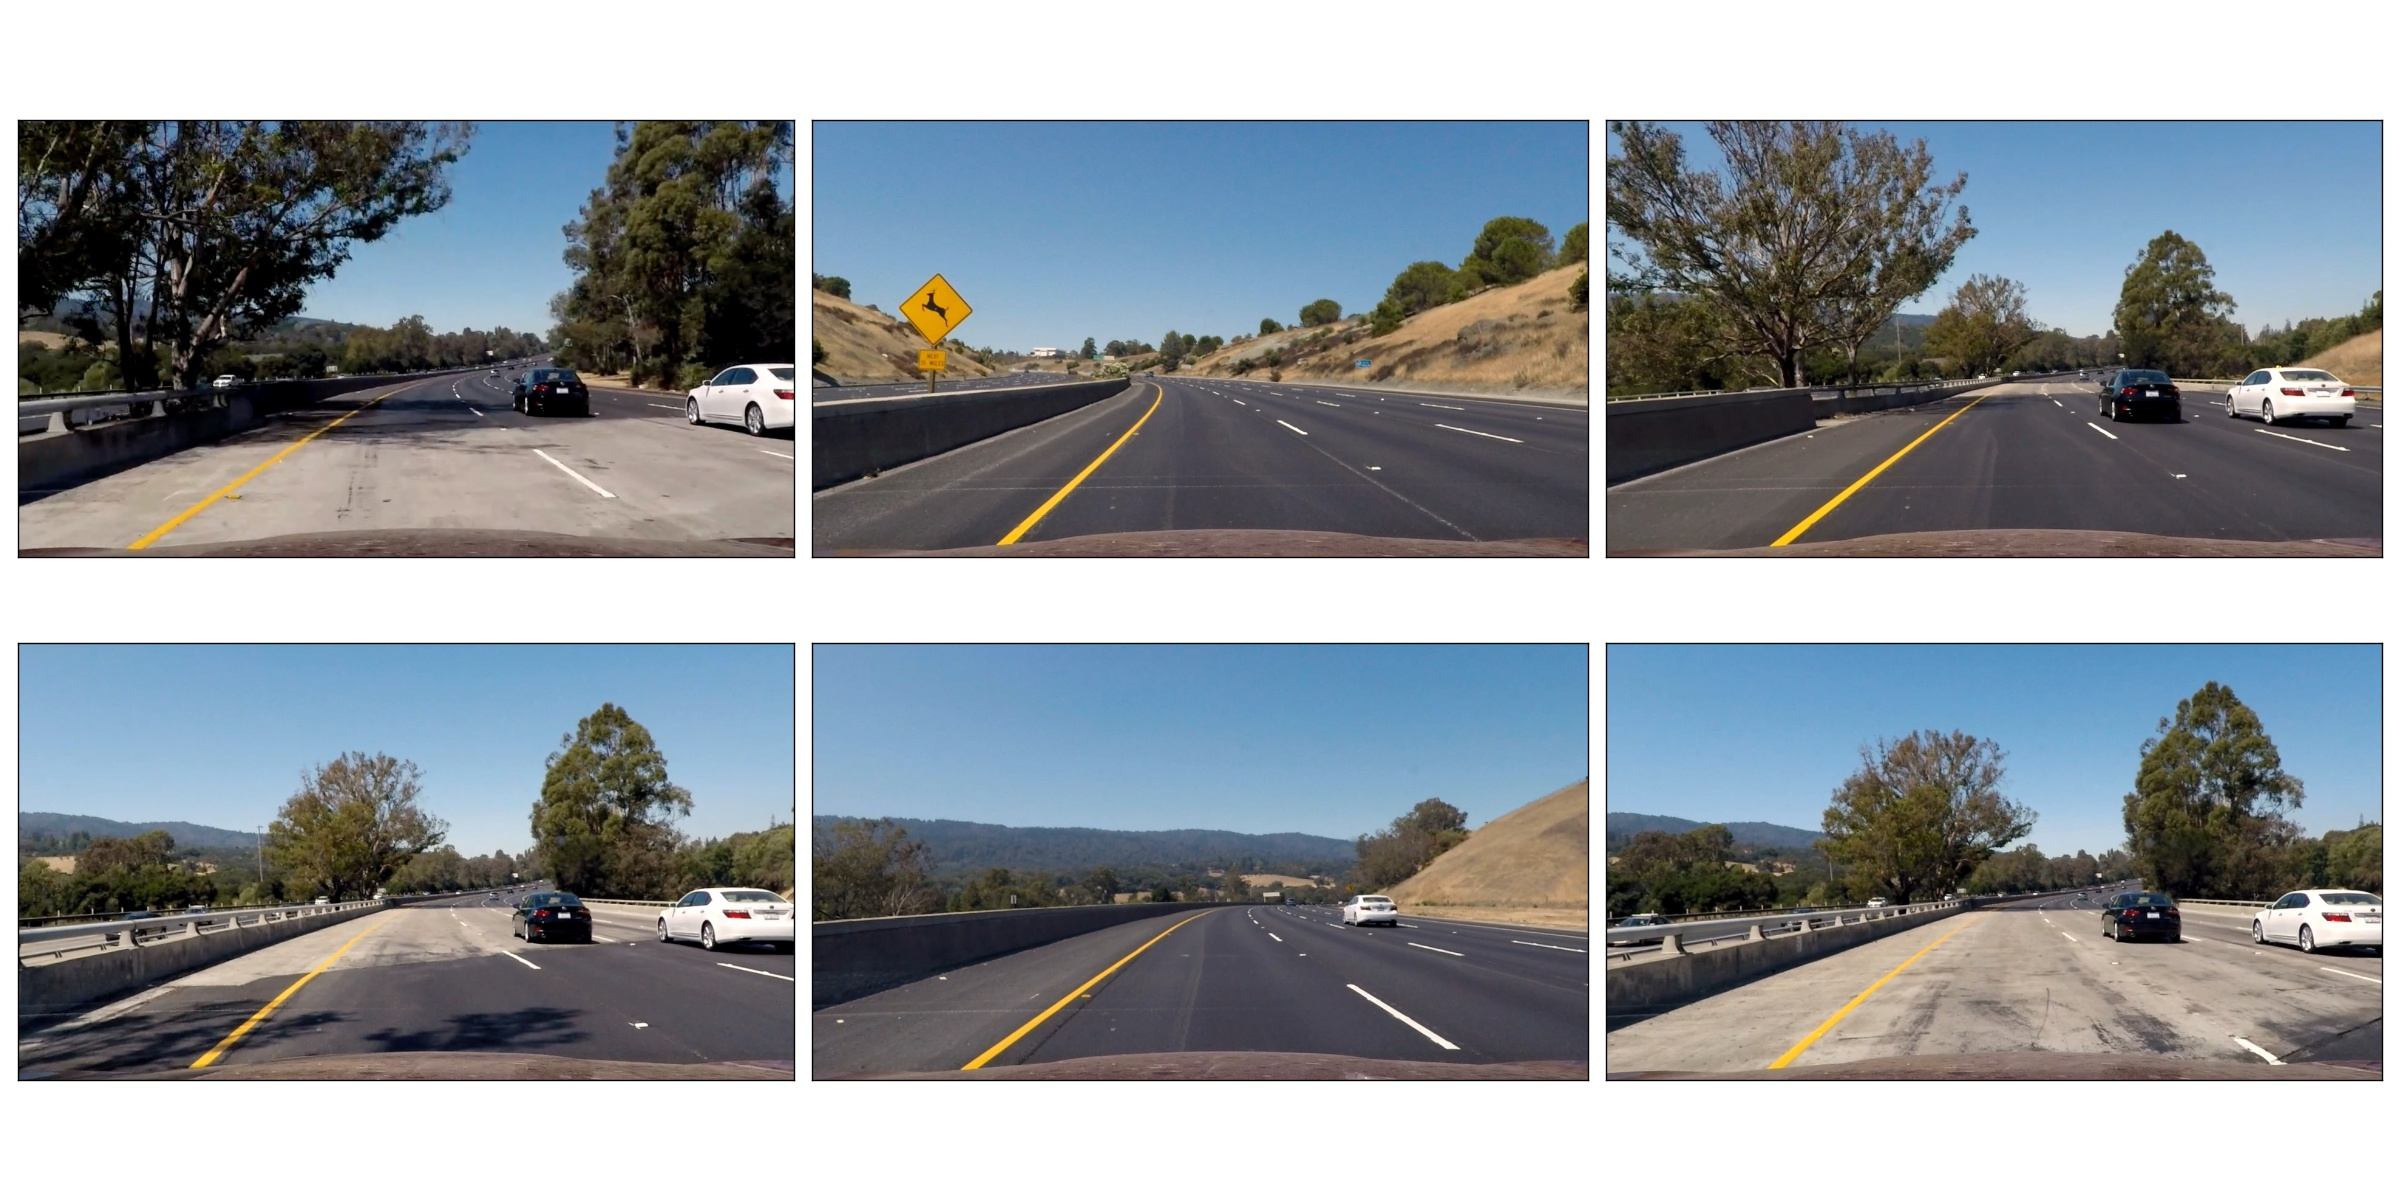
\includegraphics[width=.9\linewidth]{output_images/undistorted_test_images.jpg}

Next, we move on to perspective measurement.

\subsubsection*{Perspective Measurement}
\label{sec-2-2-3}

Perspective measurement applies to two-dimensional images taken
of three-dimensional scenes wherein objects of
interest--typically planar objects like roads--are oriented such
that their \href{http://mathworld.wolfram.com/NormalVector.html}{normal vector} is not parallel with the camera's line
of site.  Another way to put it is that the planar object is not
parallel with the \href{https://en.wikipedia.org/wiki/Image_plane}{image plane}.  While there undoubtedly are more
sophisticated, perhaps automated or semi-automated ways of doing
this, a tried-and-true method is to identify a non-rectilinear
region in the image that corresponds to the planar object of
interest (the road) and then map those to a corresponding
rectilinear region on the \href{https://en.wikipedia.org/wiki/Image_plane}{image plane}.  

The \texttt{measure\_warp} function helps measure perspective.  It takes
an image as a \href{https://docs.scipy.org/doc/numpy/reference/generated/numpy.array.html}{NumPy array} and displays the image to the user in
an interactive window.  The user only has to click four corners
in sequence for the source region and then close the interactive
window.  The destination region on the \href{https://en.wikipedia.org/wiki/Image_plane}{image plane} for now is
hard-code to a bounding box between the top and bottom of the
image and 300 pixels from the left edge and 300 pixels from the
right edge.  These values were obtained through experimentation,
and while they are not as sophisticated as giving the user
interactive control, they do have the virtue of being perfectly
rectilinear.  This is something that is difficult to achieve
manually.  Setting the src region coordinates, along with
drawing guidelines to aid the eye, is accomplished in an
event handler function for mouse-click events.  The function
returns the transformation matrix $M$ and the inverse
transformation matrix $M_{inv}$.  

\begin{verbatim}
def measure_warp(img):
    top = 0
    bottom = img.shape[0]
    def handler(e):
	if len(src)<4:
	    plt.axhline(int(e.ydata), linewidth=2, color='r')
	    plt.axvline(int(e.xdata), linewidth=2, color='r')
	    src.append((int(e.xdata),int(e.ydata)))
	if len(src)==4:
	    dst.extend([(300,bottom),(300,top),(980,top),(980,bottom)])
    was_interactive = matplotlib.is_interactive()
    if not matplotlib.is_interactive():
	plt.ion()
    fig = plt.figure()
    plt.imshow(img)
    global src                                                            
    global dst                                                            
    src = []
    dst = []
    cid1 = fig.canvas.mpl_connect('button_press_event', handler)
    cid2 = fig.canvas.mpl_connect('close_event', lambda e: e.canvas.stop_event_loop())
    fig.canvas.start_event_loop(timeout=-1)
    M = cv2.getPerspectiveTransform(np.asfarray(src, np.float32), np.asfarray(dst, np.float32))
    Minv = cv2.getPerspectiveTransform(np.asfarray(dst, np.float32), np.asfarray(src, np.float32))
    matplotlib.interactive(was_interactive)
    return M, Minv
\end{verbatim}

Like with the \texttt{get\_undistorter} function described above, we use
\href{https://www.programiz.com/python-programming/closure}{Python closures} to create a function generator called
\texttt{get\_warpers}, which measures the perspective, remembers the
transformation matrices, and then generate a new function that
uses OpenCV \href{http://docs.opencv.org/2.4/modules/imgproc/doc/geometric_transformations.html#warpperspective}{\texttt{warpPerspective}} to transform a target image.  Note
that it actually generates two functions, both to "warp" and
"unwarp" images.

\begin{verbatim}
def get_warpers(corrected_image):
    M, Minv = measure_warp(corrected_image)
    return lambda x: cv2.warpPerspective(x,
					 M,
					 x.shape[:2][::-1],
					 flags=cv2.INTER_LINEAR), \
	   lambda x: cv2.warpPerspective(x,
					 Minv,
					 x.shape[:2][::-1],
					 flags=cv2.INTER_LINEAR), M, Minv
\end{verbatim}

The following code illustrates how this is put into practice.
We get an image with the matplotlib \href{http://matplotlib.org/api/image_api.html#matplotlib.image.imread}{\texttt{imread}} function, correct
for camera distortion using the \texttt{undistort} function we
generated with the \texttt{undistorter} function created above (after
camera calibration on checkerboard images), then use
\texttt{get\_warpers} to generate both the \texttt{warp} and \texttt{unwarp}
functions.  It also returns the $M$ and $M_{inv}$ matrices as
\texttt{M} and \texttt{Minv} for good measure.

\begin{verbatim}
warp,unwarp,M,Minv = get_warpers(undistort(mpimg.imread("test_images/straight_lines2.jpg")))
\end{verbatim}

The next sequence of four figures illustrates the interactive
experiene the user has in this operation, showing step-by-step
the orthogonal guidelines that appear.  The trapezoidal area
formed bout the outside bottom two corners and the inside top
two corners of the last figure defines the source region that is
then mapped to the target region.  Again, as discussed above the
target region is a rectangle running from the bottom of the
image to the top, 300 pixels in from the left edge and 300
pixels in from the right edge.

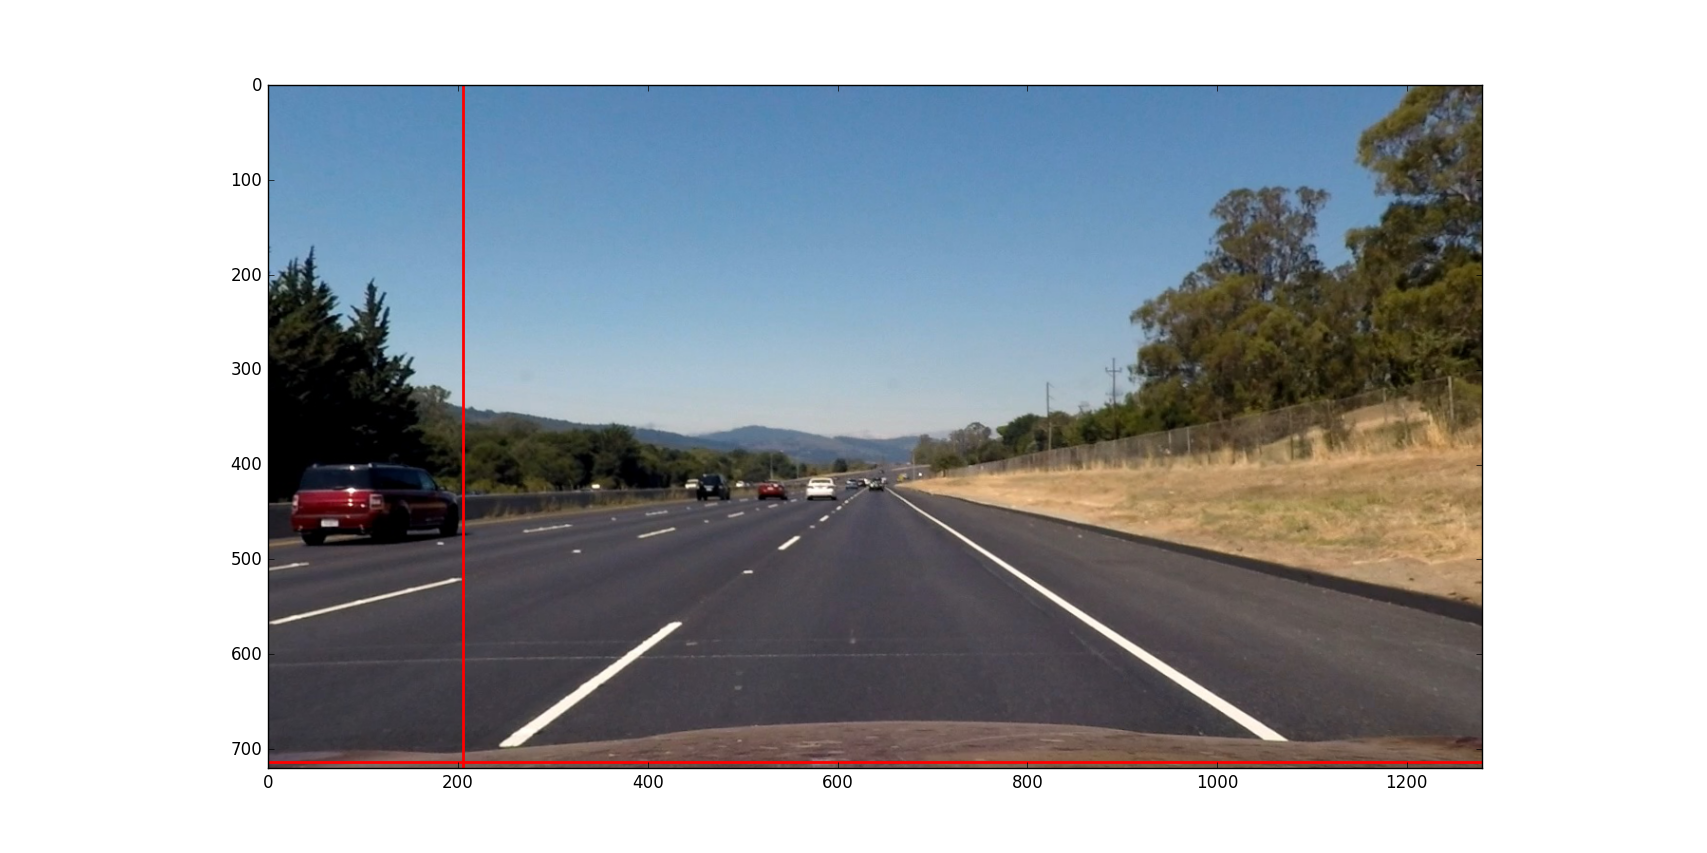
\includegraphics[width=.9\linewidth]{output_images/figure_3-1.png}

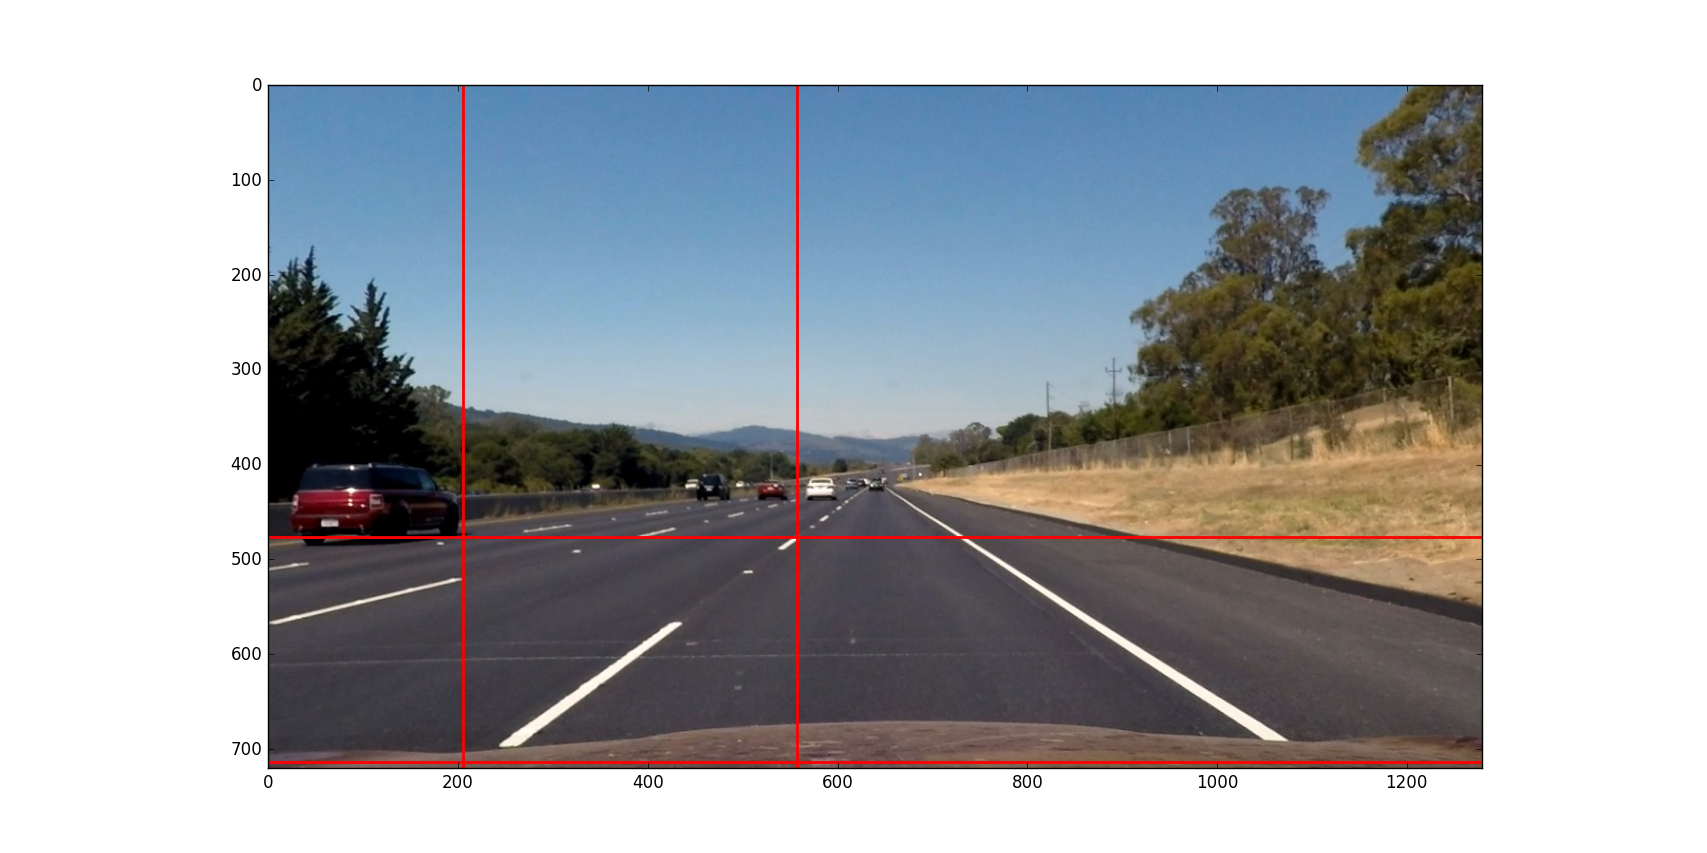
\includegraphics[width=.9\linewidth]{output_images/figure_3-2.png}

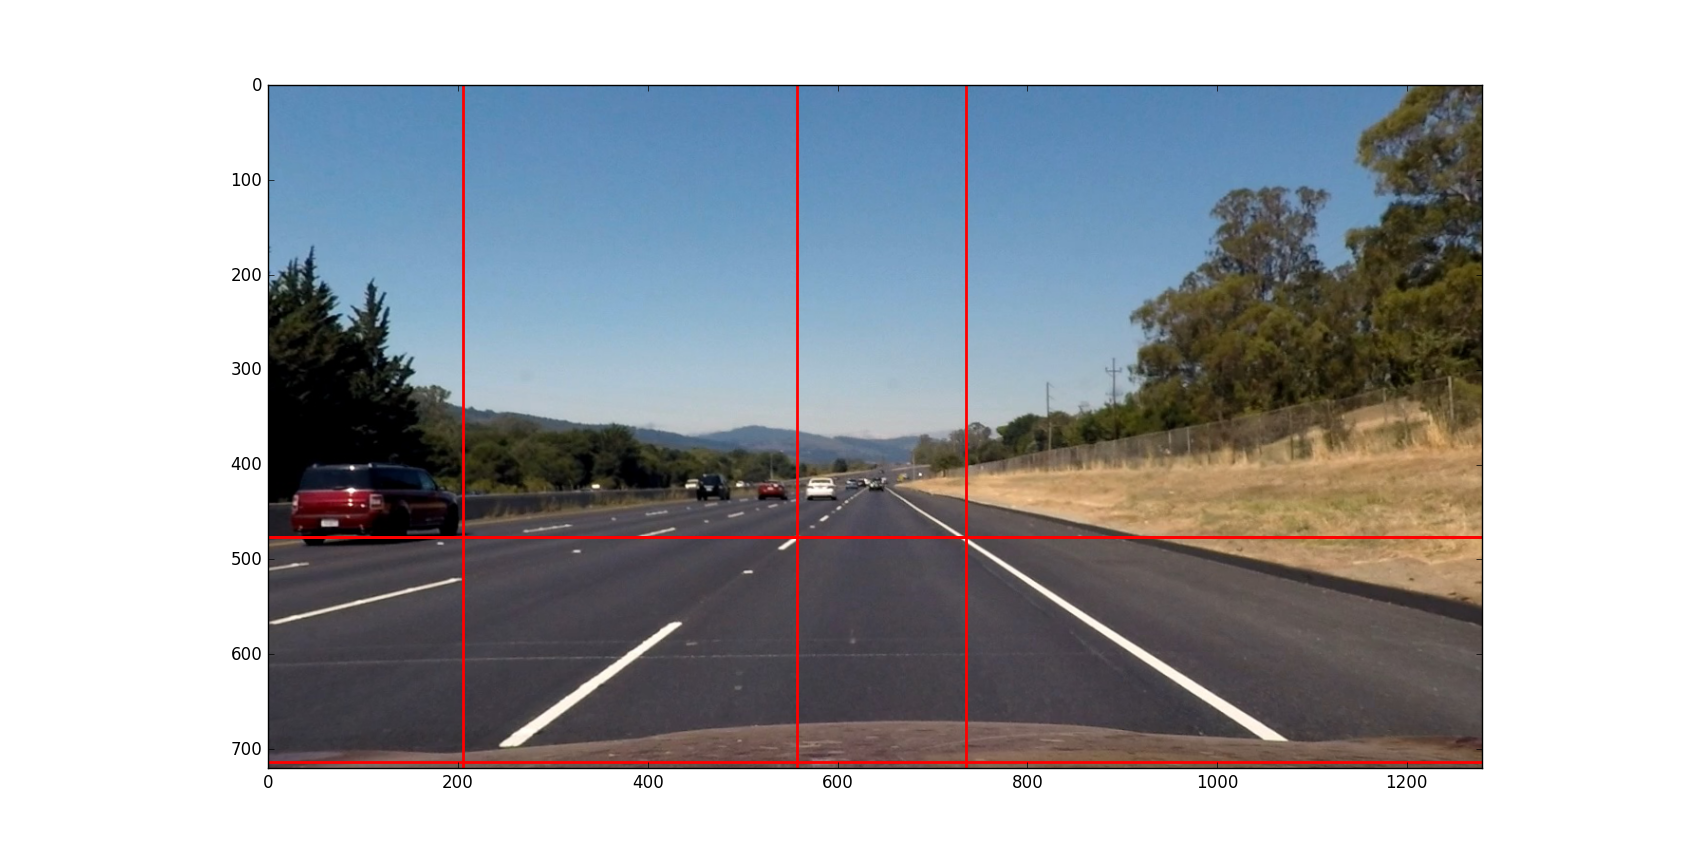
\includegraphics[width=.9\linewidth]{output_images/figure_3-3.png}

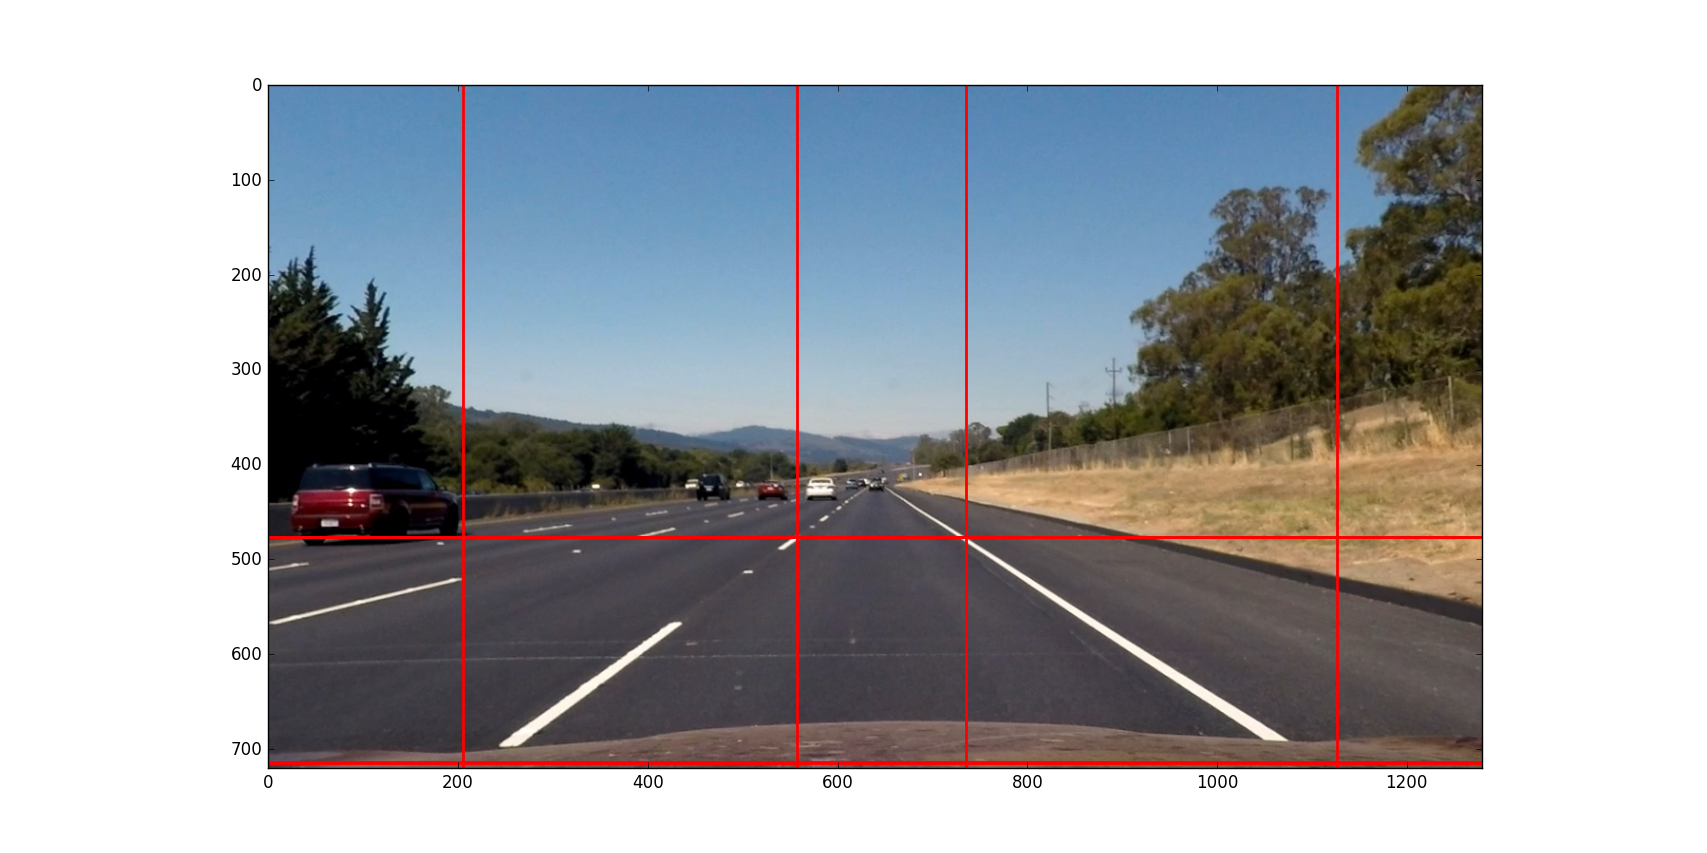
\includegraphics[width=.9\linewidth]{output_images/figure_3-4.png}

Equipped not just with an \texttt{undistort} function (obtained via
camera calibration) but also a \texttt{warp} (obtained via
perspective measurement) function, we can compose both functions
in the proper sequence (\texttt{undistort} then \texttt{warp}) and apply it to
our 6 test images.

\begin{verbatim}
visualize("output_images/warped_undistorted_test_images.jpg",
	  (warp(undistort(mpimg.imread(f))) for f in cycle(glob.glob("test_images/test*.jpg"))))
\end{verbatim}

As you can see in the following gallery we now have a
"birds-eye" (i.e. top-down) view of the road for these 6 test
images.  Note also that the perspective transform has also had
the effect of shoving out of the frame much of the extraneous
details (sky, trees, guardrails, other cars).  This is
serendipitous as it saves us from having to apply a mask just to
the lane region.  

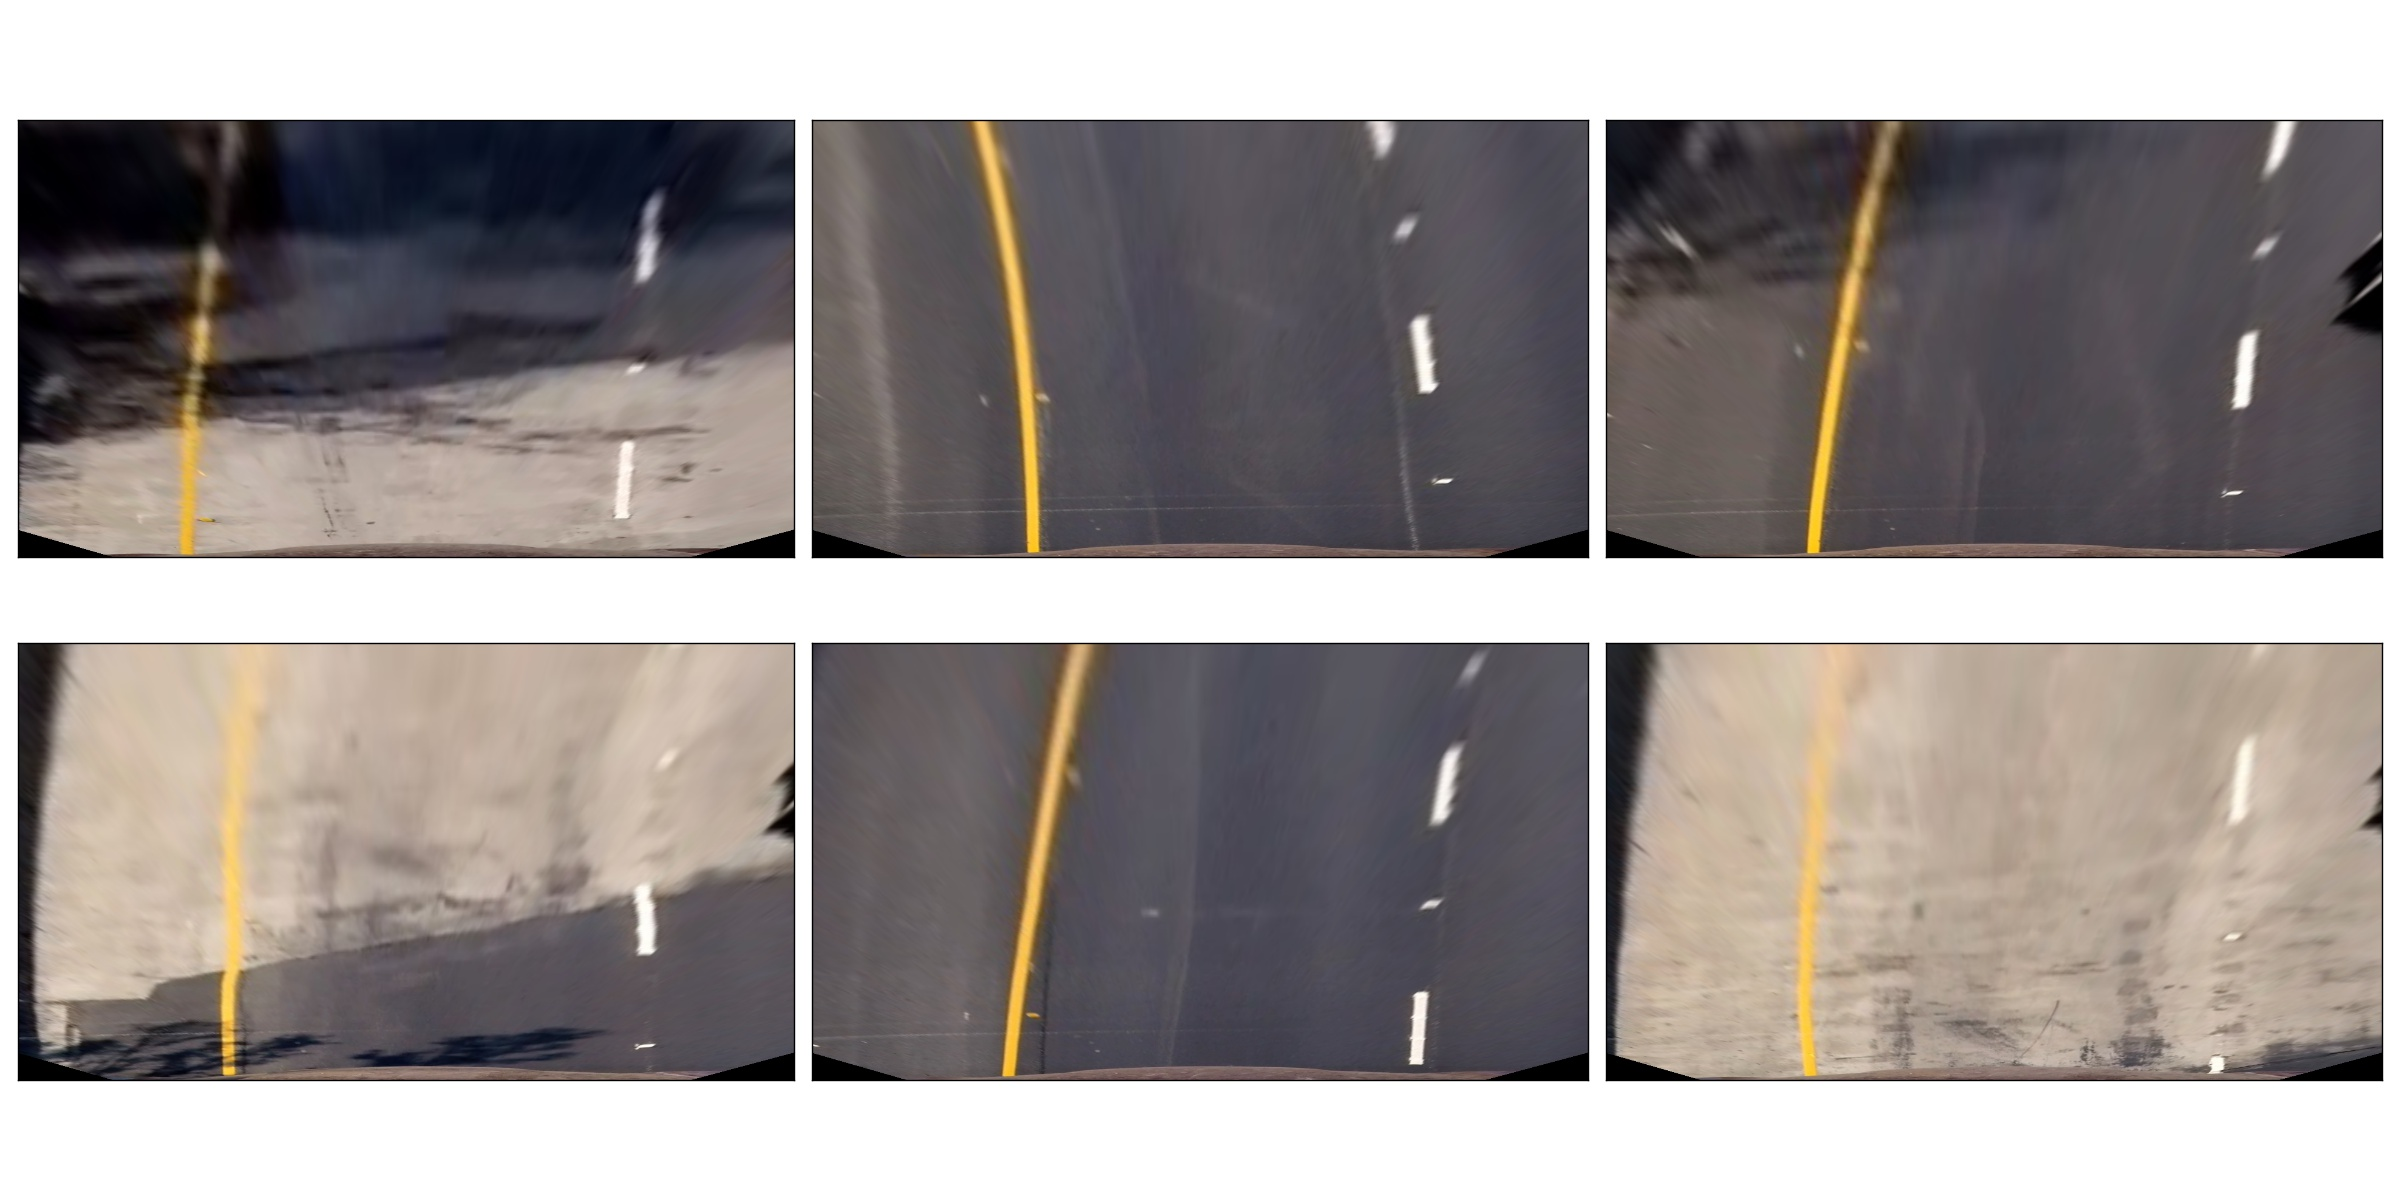
\includegraphics[width=.9\linewidth]{output_images/warped_undistorted_test_images.jpg}

Camera calibration and perspective measurement are preliminary
steps that occur before applying the processing pipeline to
images taken from the video stream.  However, they are essential
and they enable the distortion correction and perspective
transformation steps which \emph{are} part of the processing
pipeline.  Another set of essential pipeline steps involve
gradient ant color thresholds, discussed in the next sections.  

\subsubsection*{Gradient and Color Thresholds}
\label{sec-2-2-4}

Next we develop a set of useful utility functions for scaling
images, taking gradients across them, isolating different color
channels, and generating binary images.

The \texttt{scale} function scales the values of NumPy image arrays to
arbitray ranges (e.g., [0,1] or [0,255]).  The default range is
[0,255], and this is useful in order to give all images the same
scale.  Different operations (e.g., taking gradients, producing
binary images) can introduce different scales and it eases
combining and comparing images when they have the same scale.

\begin{verbatim}
def scale(img, factor=255.0):
    scale_factor = np.max(img)/factor
    return (img/scale_factor).astype(np.uint8)
\end{verbatim}

The \texttt{derivative} function uses the OpenCV \href{http://docs.opencv.org/2.4/modules/imgproc/doc/filtering.html#sobel}{\texttt{sobel}} function to
apply the \href{https://en.wikipedia.org/wiki/Sobel_operator}{Sobel operator} in order to estimate derivatives in the
$x$ and $y$ directions acoss the image.  For good measure, it
also returns both the \emph{magnitude} and the \emph{direction} of the
\href{https://en.wikipedia.org/wiki/Gradient}{gradient} computed from these derivative estimates.  

\begin{verbatim}
def derivative(img, sobel_kernel=3):
    derivx = np.absolute(cv2.Sobel(img, cv2.CV_64F, 1, 0, ksize=sobel_kernel))
    derivy = np.absolute(cv2.Sobel(img, cv2.CV_64F, 0, 1, ksize=sobel_kernel))
    gradmag = np.sqrt(derivx**2 + derivy**2)
    absgraddir = np.arctan2(derivy, derivx)
    return scale(derivx), scale(derivy), scale(gradmag), absgraddir
\end{verbatim}

The \texttt{grad} function adapts the \texttt{derivative} function to return
both the gradient \emph{magnitude} and \emph{direction}.  You might wonder
what this function adds to the \texttt{derivative} function, and that
is a valid consideration.  Largely it exists because the lecture
notes seemed to suggest that it's wortwhile to use different
kernal sizes for the Sobel operator when computing the gradient
direction.  In hindsight it's not clear this function really is
adding value and it may be removed in future versions.

\begin{verbatim}
def grad(img, k1=3, k2=15):
    _,_,g,_ = derivative(img, sobel_kernel=k1)
    _,_,_,p = derivative(img, sobel_kernel=k2)
    return g,p
\end{verbatim}

The \texttt{hls\_select} function is a convenience that fans out the
three channels of the \href{https://en.wikipedia.org/wiki/HSL_and_HSV}{HLS color-space} into separate NumPy
arrays.  

\begin{verbatim}
def hls_select(img):
    hsv = cv2.cvtColor(img, cv2.COLOR_RGB2HLS).astype(np.float)
    h = hsv[:,:,0]
    l = hsv[:,:,1]
    s = hsv[:,:,2]
    return h,l,s
\end{verbatim}

The \texttt{rgb\_select} function is another convenience that returns
the three channels of the \href{https://en.wikipedia.org/wiki/RGB_color_space}{RGB color-space}.

\begin{verbatim}
def rgb_select(img):
    rgb = img
    r = rgb[:,:,0]
    g = rgb[:,:,1]
    b = rgb[:,:,2]
    return r,g,b
\end{verbatim}

The \texttt{threshold} function is a convenience that applies
\texttt{thresh\_min} and \texttt{thresh\_max} \emph{min-max} values and logical
operations in order to obtain "binary" images.  Binary images
have activated pixels (non-zero values) for desired features.

\begin{verbatim}
def threshold(img, thresh_min=0, thresh_max=255):
    binary_output = np.zeros_like(img)
    binary_output[(img >= thresh_min) & (img <= thresh_max)] = 1
    return binary_output
\end{verbatim}

The \texttt{land} and \texttt{lor} functions are conveniences for combining
binary images, either with logical \href{https://en.wikipedia.org/wiki/Logical_conjunction}{conjunction} or \href{https://en.wikipedia.org/wiki/Logical_disjunction}{disjunction},
respectively.  

\begin{verbatim}
land = lambda *x: np.logical_and.reduce(x)
lor = lambda *x: np.logical_or.reduce(x)
\end{verbatim}

There are various ways of doing this.  Another way is to stack
binary image arrays using the NumPy \href{https://docs.scipy.org/doc/numpy/reference/generated/numpy.stack.html}{\texttt{stack}} function and then
interleave various combinations of such interleavings along with
the NumPy \href{https://docs.scipy.org/doc/numpy/reference/generated/numpy.any.html#numpy-any}{\texttt{any}} function and \href{https://docs.scipy.org/doc/numpy/reference/generated/numpy.all.html#numpy-all}{\texttt{all}} function.  It's a clever
approach, but I find that applying the NumPy \href{https://docs.scipy.org/doc/numpy/reference/generated/numpy.logical_and.html#numpy-logical-and}{\texttt{logical\_and}} and
\href{https://docs.scipy.org/doc/numpy/reference/generated/numpy.logical_or.html#numpy-logical-or}{\texttt{logical\_or}} functions as above leads to less typing.  

The \texttt{highlight} function composes the color channel selection,
gradient estimation, binary threshold, logical composition, and
scaling operations to an input image in order to "highlight" the
desired features, such as lane lines.  Note that distortion
correction and perspective transformation are considered outside
the scope of this function.  In a real pipeline, those two
operations almost certainly should be applied to an image before
presenting it to the \texttt{highlight} function.  In general, they
need not be, which can be useful during the exploratory phase of
pipeline development.

\begin{verbatim}
def highlight(img):
    r,g,b = rgb_select(img)
    h,l,s = hls_select(img)
    o01 = threshold(r, 200, 255)
    o02 = threshold(g, 200, 255)
    o03 = threshold(s, 200, 255)
    return scale(lor(land(o01,o02),o03))
\end{verbatim}

In fact, the highlight and undistort operations are combined
\emph{without} perspective transform in the next gallery of 6 test
images.  This is an example of a common iteration pattern while
exploring pipeline options.

\begin{verbatim}
visualize("output_images/binary_undistorted_test_images.jpg",
	  (highlight(undistort(mpimg.imread(f))) for f in cycle(glob.glob("test_images/test*.jpg"))))
\end{verbatim}

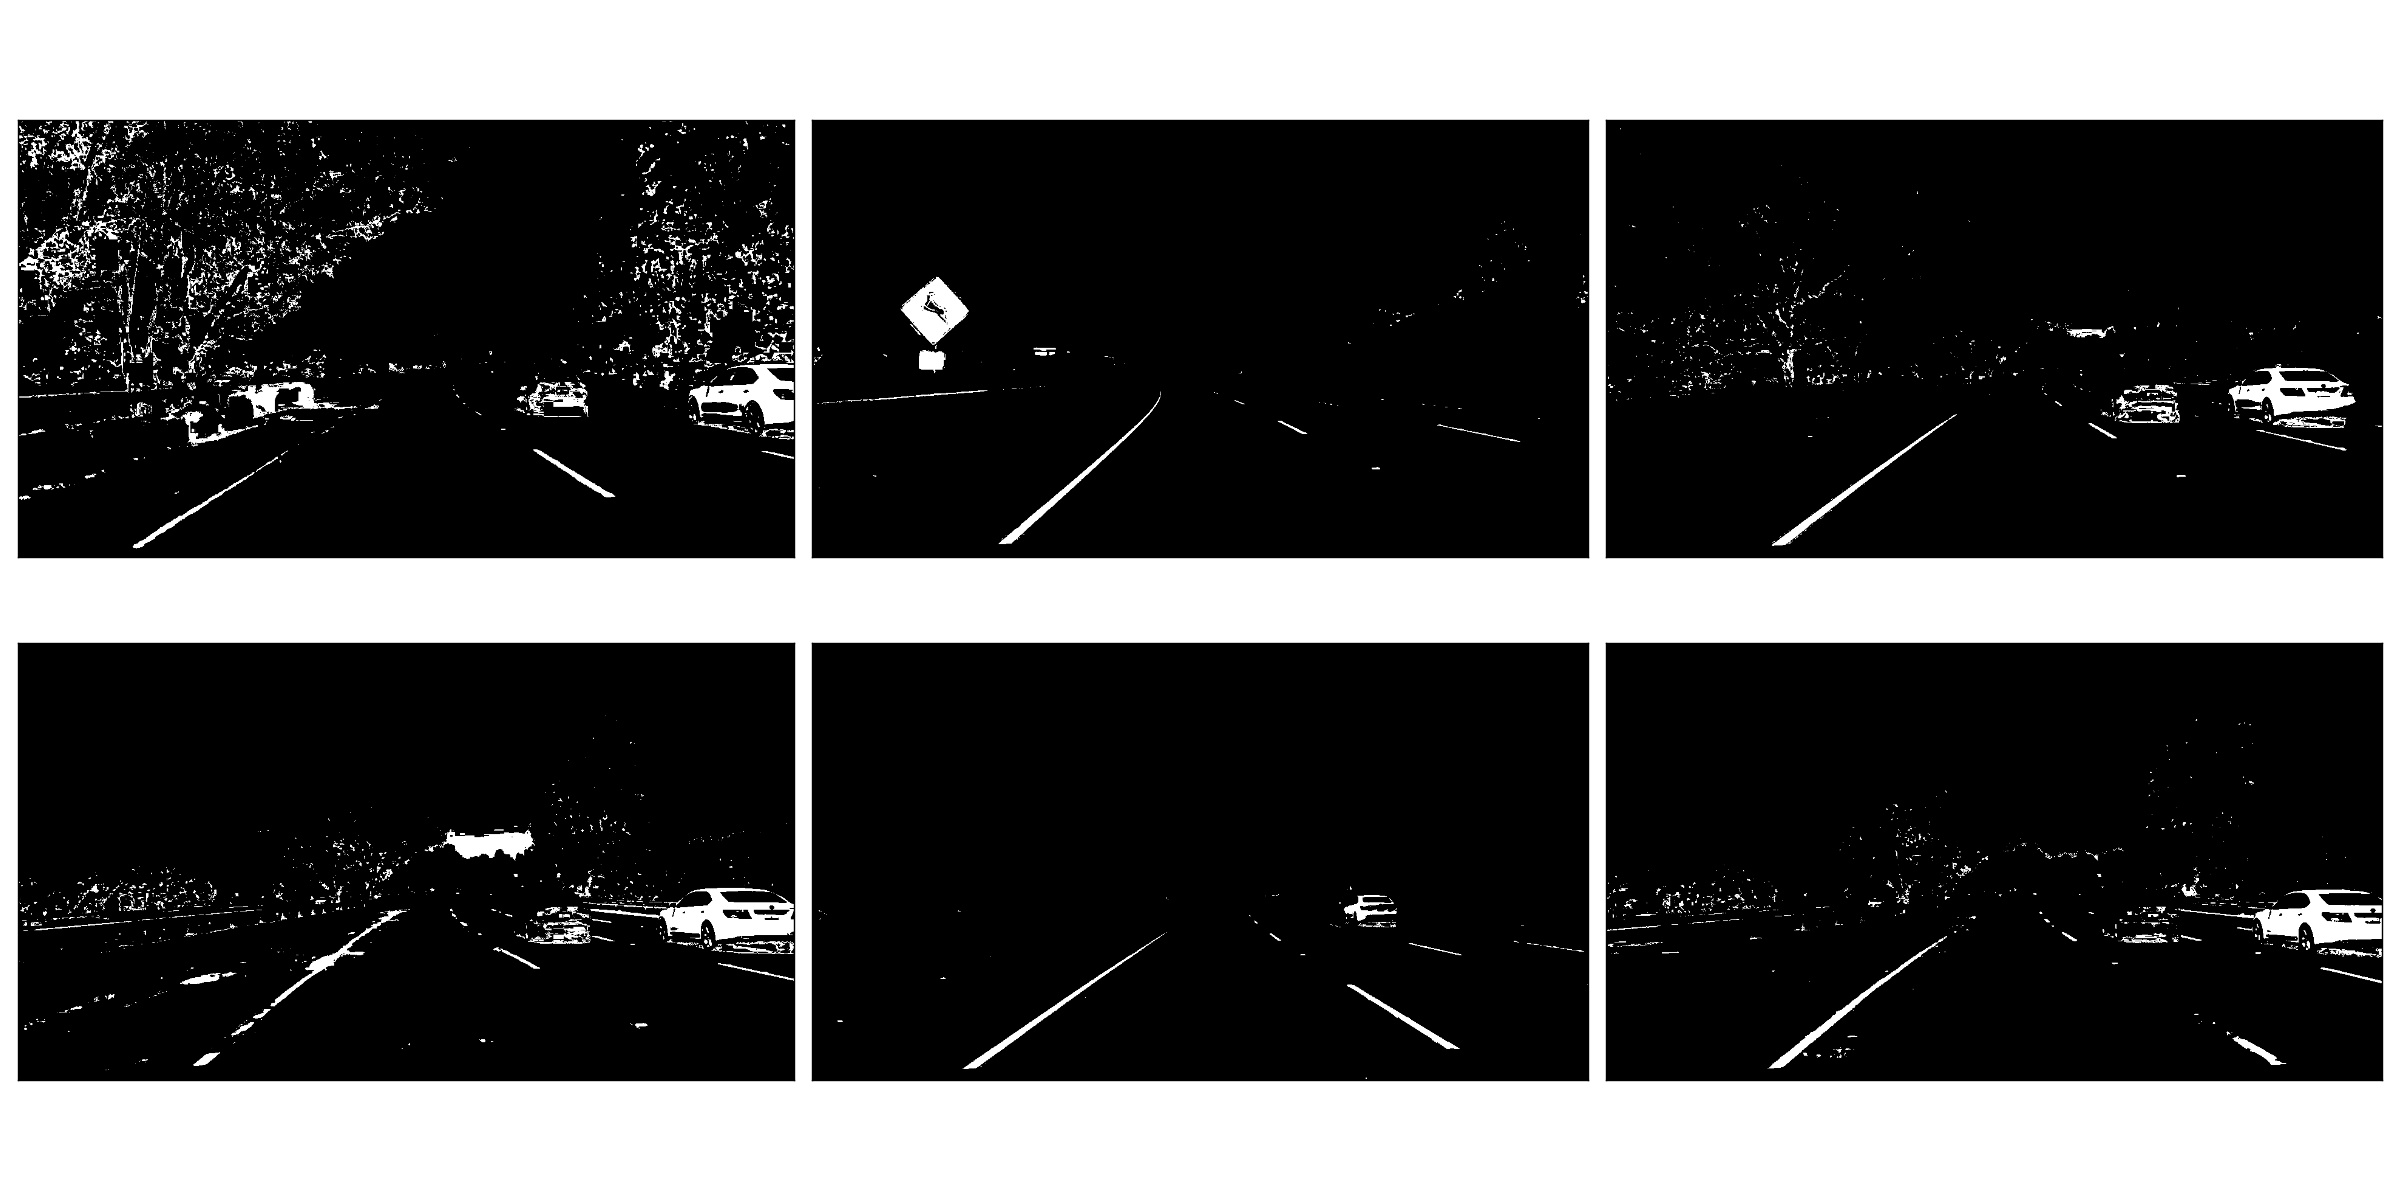
\includegraphics[width=.9\linewidth]{output_images/binary_undistorted_test_images.jpg}

\subsubsection*{Perspective Transform}
\label{sec-2-2-5}

Armed with a pipeline which, based on the 6 test images, we
believe may be a good candidate for detecting lane lines, we
then see what the pipeline-processed test images look like after
transforming them to a "bird's-eye" view.

\begin{verbatim}
visualize("output_images/warped_binary_undistorted_images.jpg",
	  (warp(highlight(undistort(mpimg.imread(f)))) for f in cycle(glob.glob("test_images/test*.jpg"))))
\end{verbatim}

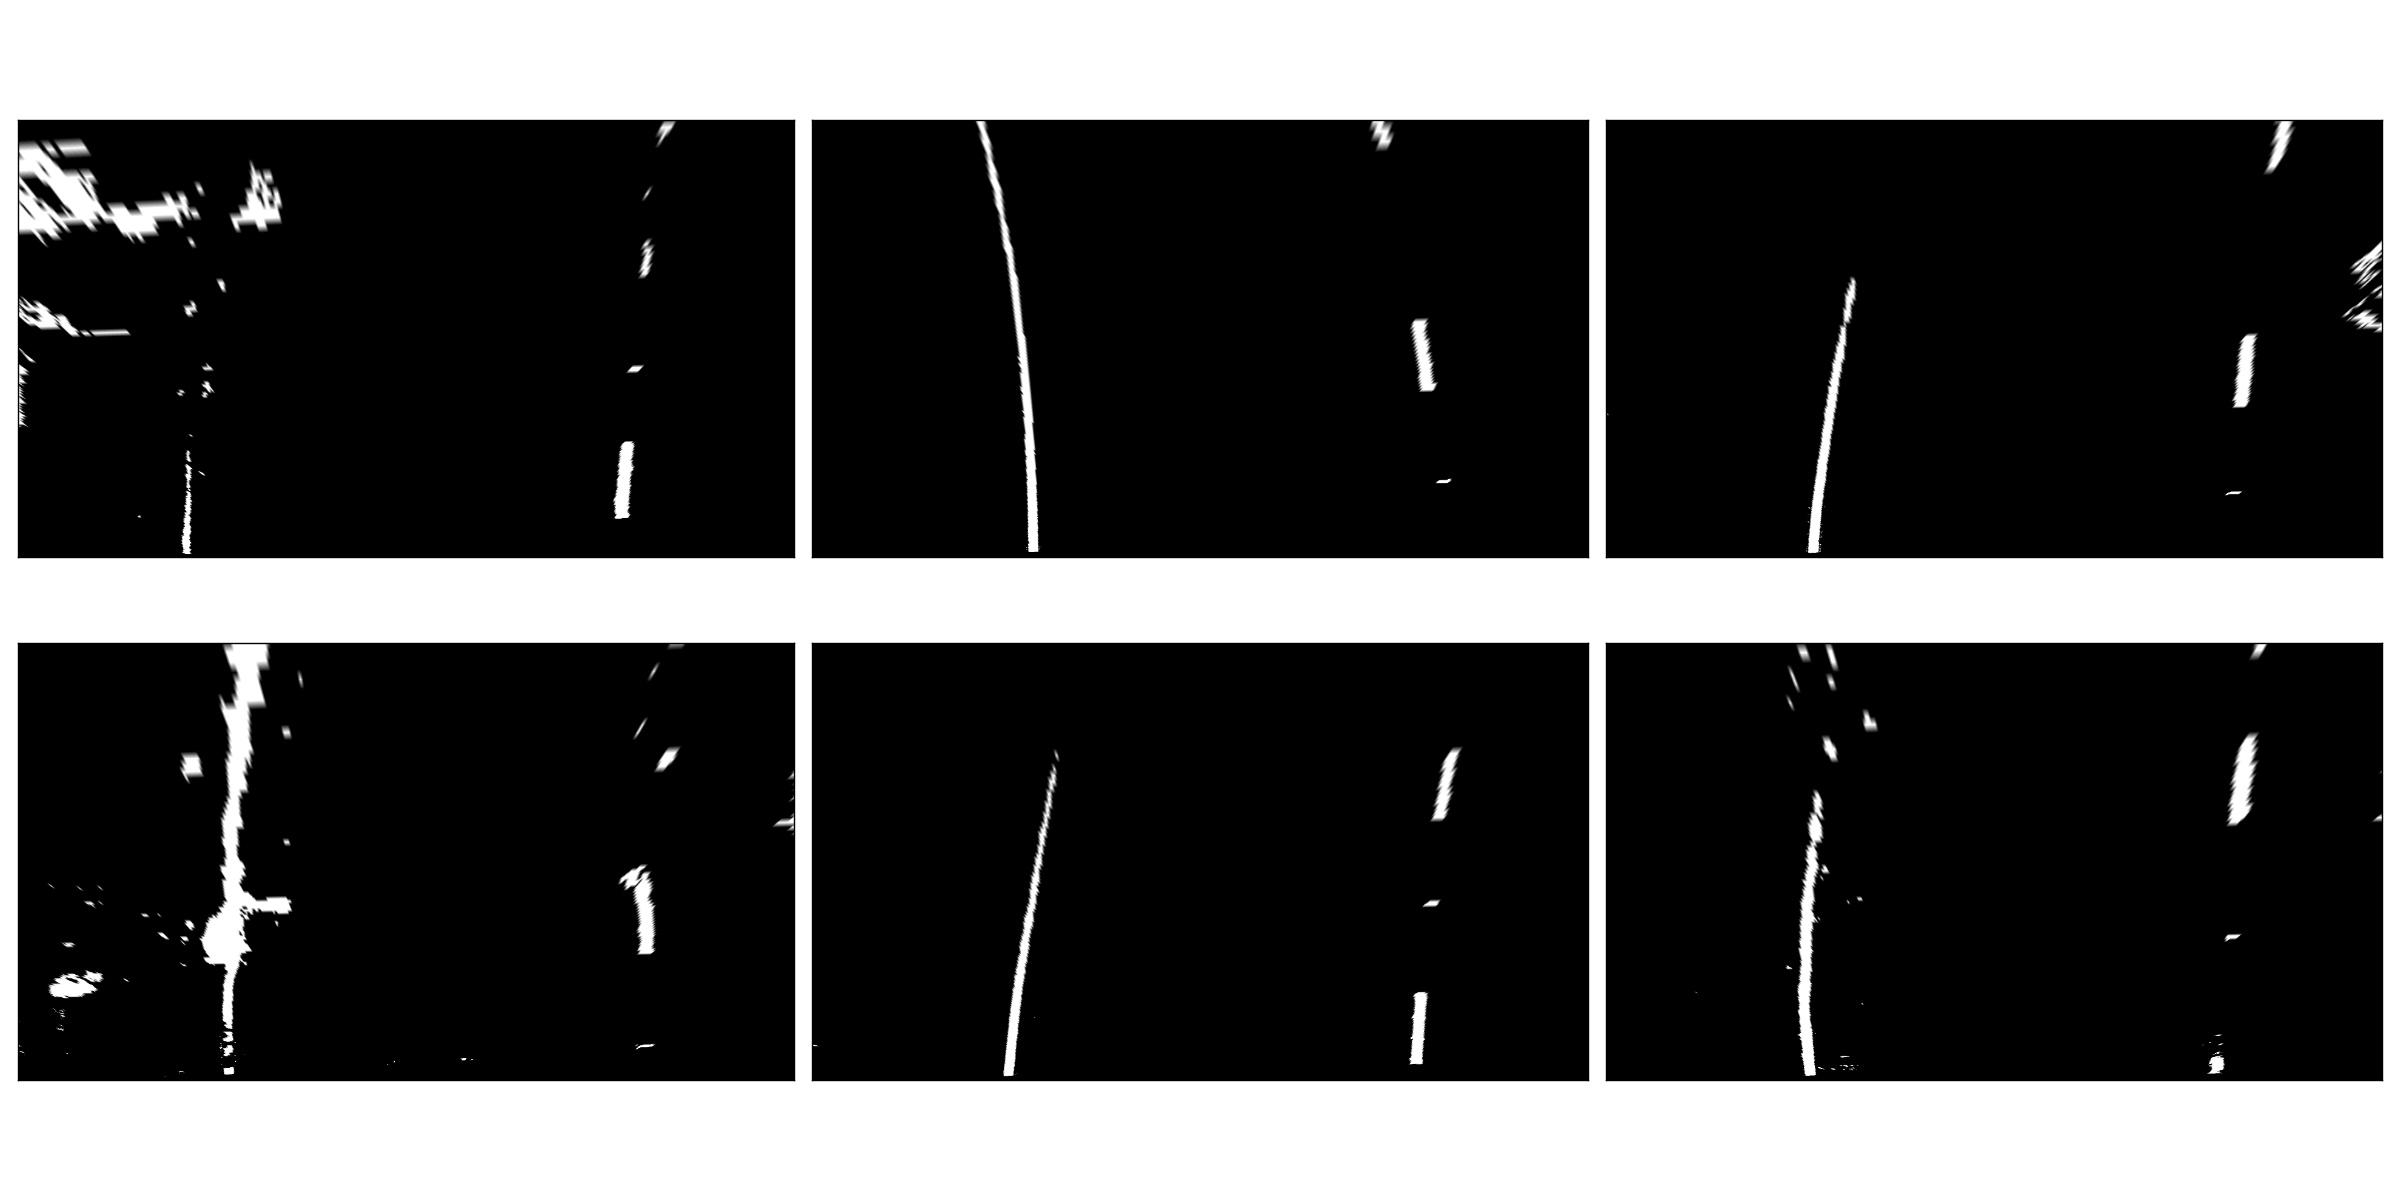
\includegraphics[width=.9\linewidth]{output_images/warped_binary_undistorted_images.jpg}

\subsubsection*{Lane-Finding}
\label{sec-2-2-6}

Lane-line detection can be done somewhat laboriously--but
perhaps more accurately--using a "sliding window" technique.
Roughly, the algorithm implemented in
\texttt{detect\_lines\_sliding\_window} below has these steps, also
discussed in the code comments.

\begin{enumerate}
\item Take a histogram across the bottom of the image.
\item Find the histogram peaks to identify the lane lines at the
bottom of the image.
\item Divide the image into a vertical stack of narrow horizontal
slices.
\item Select activated pixels (remember, the input is a binary
image) only in a "neighborhood" of our current estimate of
the lane position.  This neighborhood is the "sliding
window."  To bootstrap the process, our initial estimate of
the lane line location is taken from the histogram peak steps
listed above.  Essentially, we are removing "outliers"
\item Estimate the new lane-line location for this window from the
mean of the pixels falling within the sliding window.
\item March vertically up through the stack, repeating this process.
\item Select all activated pixels within all of our sliding windows.
\item Fit a quadratic function to these selected pixels, obtaining
model parameters.
\end{enumerate}

The model parameters essentially represent the detected
lane-line.  We do this both for the left and right lines.
Moreover, we also perform a few somewhat ancillary operations
while we're at it.

\begin{enumerate}
\item Draw the slinding windows, the selected pixels, and the
modeled quadratic curve onto a copy of the image.
\item Recompute the function fit after scaling the pixel locations
to real world values, then use these model fit parameters to
compute a real-world radius of curvature for both lanes.
\end{enumerate}

The function \texttt{detect\_lines\_sliding\_window} returns quite a few values:

\begin{enumerate}
\item left lane fit parameters
\item right lane fit parameters
\item left lane fit residuals
\item right lane fit residuals
\item left lane real-world radius (in meters)
\item right lane real-world radius (in meters)
\item annotated image, with sliding windows, selected pixels, and
modeled curves
\end{enumerate}

\begin{verbatim}
def detect_lines_sliding_window(warped_binary):
    # Assuming you have created a warped binary image called "warped_binary"
    # Take a histogram of the bottom half of the image
    histogram = np.sum(warped_binary[warped_binary.shape[0]/2:,:], axis=0)
    # Create an output image to draw on and  visualize the result
    out_img = np.dstack((warped_binary, warped_binary, warped_binary))*255
    # Find the peak of the left and right halves of the histogram
    # These will be the starting point for the left and right lines
    midpoint = np.int(histogram.shape[0]/2)
    leftx_base = np.argmax(histogram[:midpoint])
    rightx_base = np.argmax(histogram[midpoint:]) + midpoint
    # Choose the number of sliding windows
    nwindows = 9
    # Set height of windows
    window_height = np.int(warped_binary.shape[0]/nwindows)
    # Identify the x and y positions of all nonzero pixels in the image
    nonzero = warped_binary.nonzero()
    nonzeroy = np.array(nonzero[0])
    nonzerox = np.array(nonzero[1])
    # Current positions to be updated for each window
    leftx_current = leftx_base
    rightx_current = rightx_base
    # Set the width of the windows +/- margin
    margin = 100
    # Set minimum number of pixels found to recenter window
    minpix = 50
    # Create empty lists to receive left and right lane pixel indices
    left_lane_inds = []
    right_lane_inds = []
    # Step through the windows one by one
    for window in range(nwindows):
	# Identify window boundaries in x and y (and right and left)
	win_y_low = warped_binary.shape[0] - (window+1)*window_height
	win_y_high = warped_binary.shape[0] - window*window_height
	win_xleft_low = leftx_current - margin
	win_xleft_high = leftx_current + margin
	win_xright_low = rightx_current - margin
	win_xright_high = rightx_current + margin
	# Draw the windows on the visualization image
	cv2.rectangle(out_img,(win_xleft_low,win_y_low),(win_xleft_high,win_y_high),(0,255,0), 2) 
	cv2.rectangle(out_img,(win_xright_low,win_y_low),(win_xright_high,win_y_high),(0,255,0), 2) 
	# Identify the nonzero pixels in x and y within the window
	good_left_inds = ((nonzeroy >= win_y_low) & (nonzeroy < win_y_high) & (nonzerox >= win_xleft_low) & (nonzerox < win_xleft_high)).nonzero()[0]
	good_right_inds = ((nonzeroy >= win_y_low) & (nonzeroy < win_y_high) & (nonzerox >= win_xright_low) & (nonzerox < win_xright_high)).nonzero()[0]
	# Append these indices to the lists
	left_lane_inds.append(good_left_inds)
	right_lane_inds.append(good_right_inds)
	# If you found > minpix pixels, recenter next window on their mean position
	if len(good_left_inds) > minpix:
	    leftx_current = np.int(np.mean(nonzerox[good_left_inds]))
	if len(good_right_inds) > minpix:        
	    rightx_current = np.int(np.mean(nonzerox[good_right_inds]))
    # Concatenate the arrays of indices
    left_lane_inds = np.concatenate(left_lane_inds)
    right_lane_inds = np.concatenate(right_lane_inds)
    # Extract left and right line pixel positions
    leftx = nonzerox[left_lane_inds]
    lefty = nonzeroy[left_lane_inds] 
    rightx = nonzerox[right_lane_inds]
    righty = nonzeroy[right_lane_inds] 
    # Fit a second order polynomial to each
    left_fit,left_res,_,_,_ = np.polyfit(lefty, leftx, 2, full=True)
    right_fit,right_res,_,_,_ = np.polyfit(righty, rightx, 2, full=True)
    # Generate x and y values for plotting
    ploty = np.linspace(0, warped_binary.shape[0]-1, warped_binary.shape[0] )
    left_fitx = left_fit[0]*ploty**2 + left_fit[1]*ploty + left_fit[2]
    right_fitx = right_fit[0]*ploty**2 + right_fit[1]*ploty + right_fit[2]
    out_img[nonzeroy[left_lane_inds], nonzerox[left_lane_inds]] = [255, 0, 0]
    out_img[nonzeroy[right_lane_inds], nonzerox[right_lane_inds]] = [0, 0, 255]
    out_img[ploty.astype('int'),left_fitx.astype('int')] = [0, 255, 255]
    out_img[ploty.astype('int'),right_fitx.astype('int')] = [0, 255, 255]
    y_eval = warped_binary.shape[0]
    # Define conversions in x and y from pixels space to meters
    ym_per_pix = 30/720 # meters per pixel in y dimension
    xm_per_pix = 3.7/700 # meters per pixel in x dimension
    # Fit new polynomials to x,y in world space
    left_fit_cr = np.polyfit(lefty*ym_per_pix, leftx*xm_per_pix, 2)
    right_fit_cr = np.polyfit(righty*ym_per_pix, rightx*xm_per_pix, 2)
    # Calculate the new radii of curvature
    left_curverad = ((1 + (2*left_fit_cr[0]*y_eval*ym_per_pix + left_fit_cr[1])**2)**1.5) / np.absolute(2*left_fit_cr[0])
    right_curverad = ((1 + (2*right_fit_cr[0]*y_eval*ym_per_pix + right_fit_cr[1])**2)**1.5) / np.absolute(2*right_fit_cr[0])
    return left_fit, right_fit, np.sqrt(left_fit[1]/len(leftx)), np.sqrt(right_fit[1]/len(rightx)), left_curverad, right_curverad, out_img
\end{verbatim}

The following figures shows the annotated image resulting from
applying this particular lane-finding algorithm to our 6 test
images, after distortion correction, highlighting, and
perspective transformation.

\begin{verbatim}
visualize("output_images/detected_lines_test_images.jpg",
	  (detect_lines_sliding_window(warp(highlight(undistort(mpimg.imread(f)))))[6] for f in cycle(glob.glob("test_images/test*.jpg"))))
\end{verbatim}

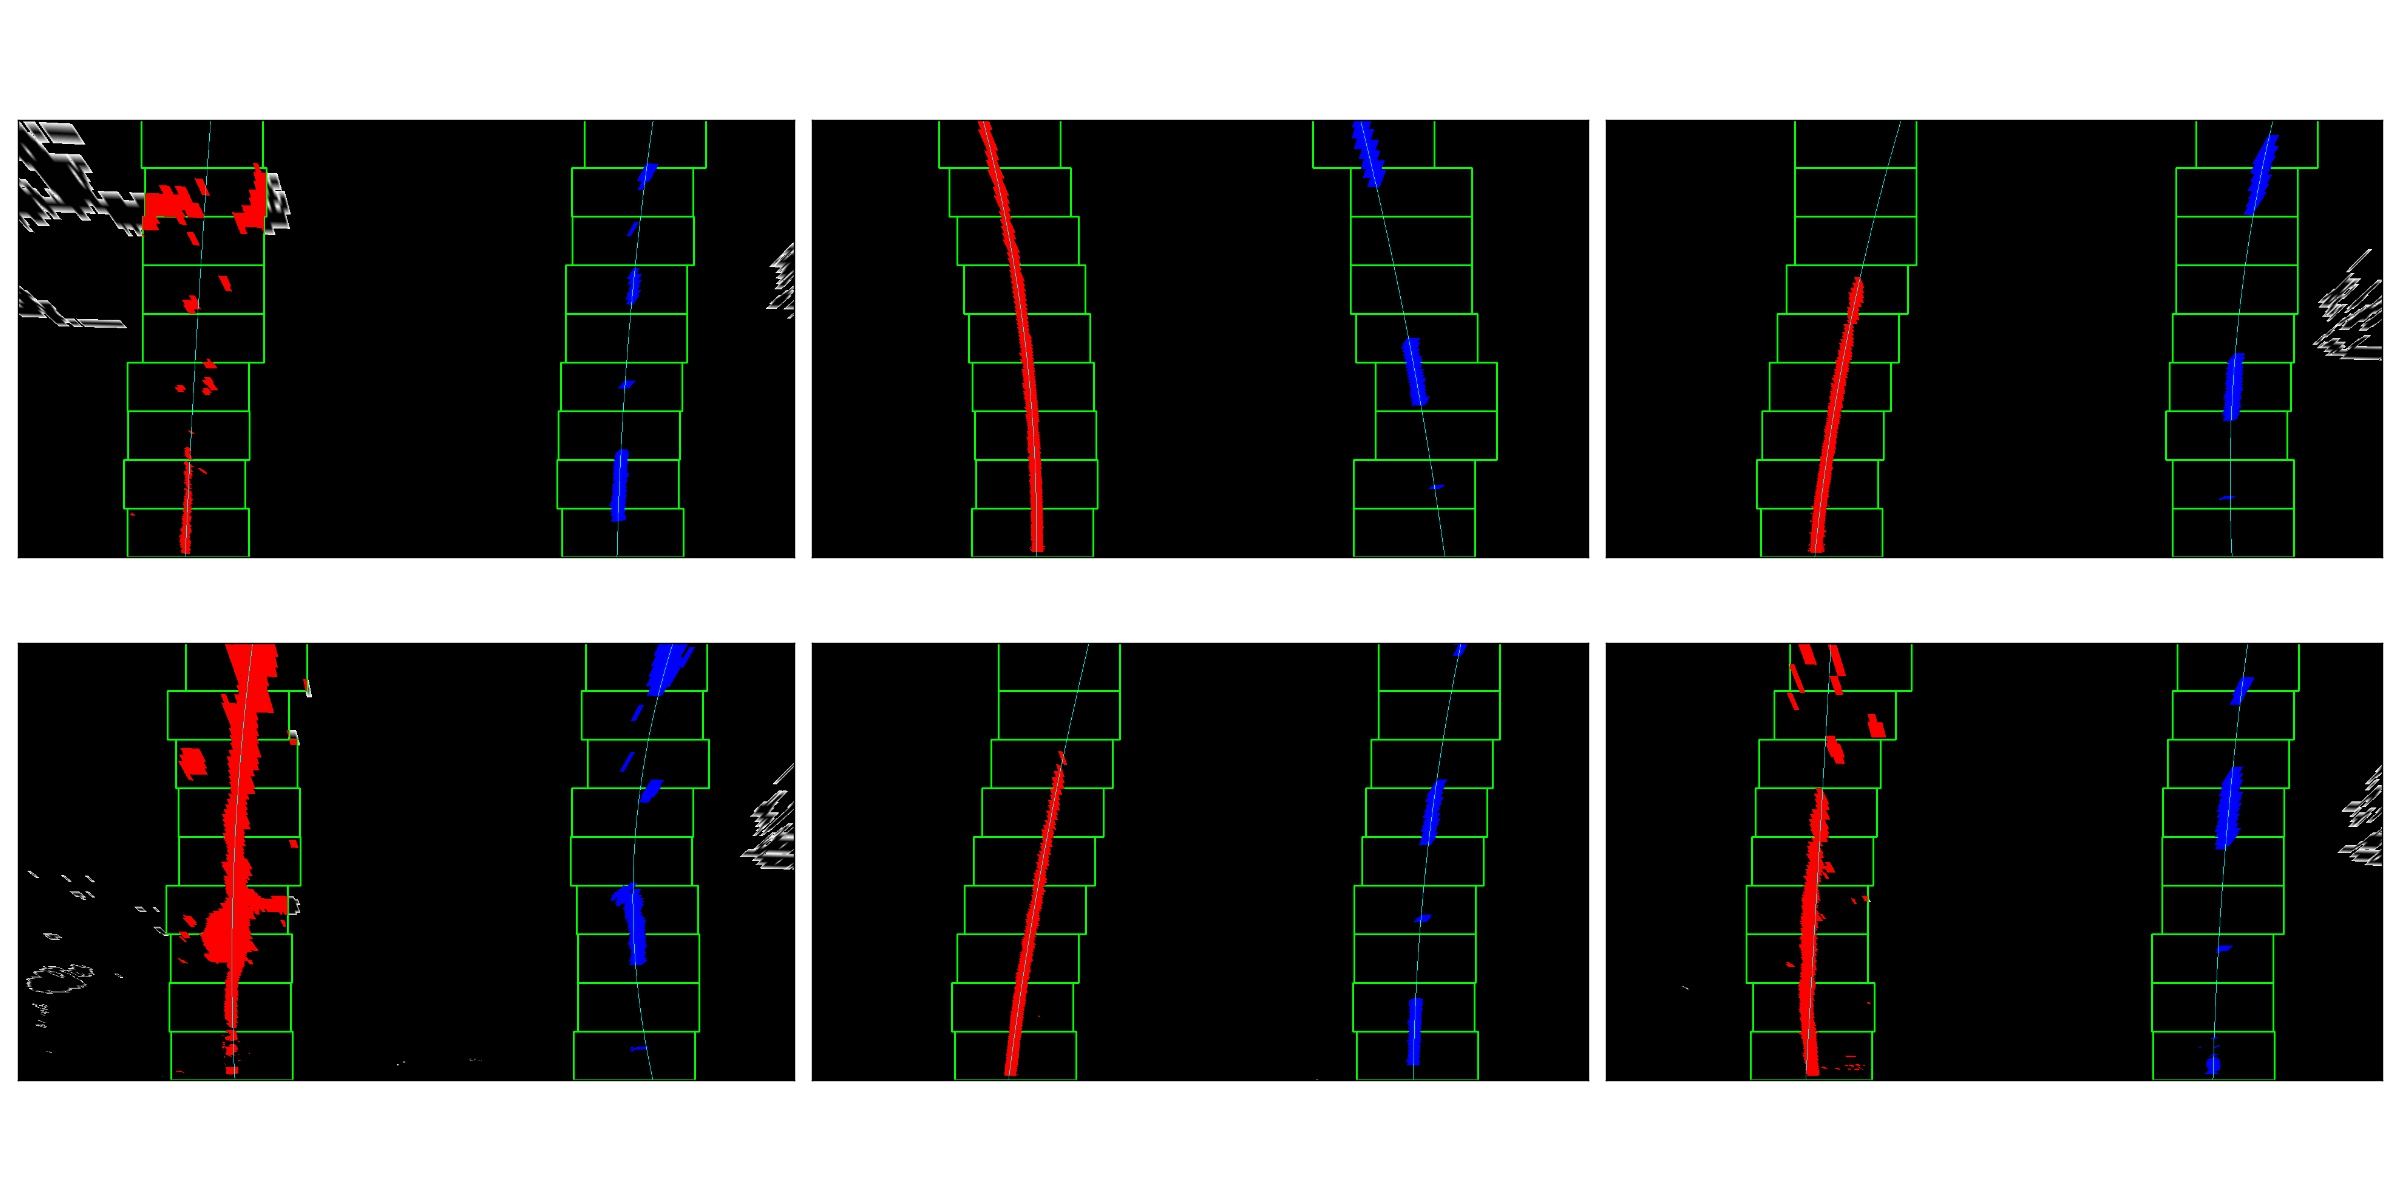
\includegraphics[width=.9\linewidth]{output_images/detected_lines_test_images.jpg}

Armed with a good estimate for the current lane-line locations
and with the observation that the lanes do not change
dramatically from one frame to the next, we can implement an
optimization.  Recall that the \emph{only reason} for the sliding
window algorithm is to remove outliers.  If we were content just
to fit all of the pixels, good or bad, we would only need to
divide the frame into a left half and a right half and then fit
the quadratic curves straight away.  However, guided by the
lecture we chose to remove outliers.  That requires a good guess
for where the lane line is, which almost inevitably leads us to
the sliding window technique.

The \texttt{detect\_lines} function takes \texttt{left\_fit} and \texttt{right\_fit}
arguments, which are good estimates of the model fit parameters
obtained from the previous video frame.  It then selects pixels
in the neighborhood of the curve computed for these parameters,
and fits new parameters for the current frame from the selected
pixels.  Thus, it avoids the labor of the sliding window
technique so long as one already has a good estimate of the
model fit parameters.  Note that, because this function does
\emph{not} apply the sliding window technique, it cannot draw the
sliding windows.  Therefore, the last parameter returned isn
\texttt{None}.  

\begin{verbatim}
def detect_lines(warped_binary, left_fit, right_fit):
    # from the next frame of video (also called "binary_warped")
    # It's now much easier to find line pixels!
    nonzero = warped_binary.nonzero()
    nonzeroy = np.array(nonzero[0])
    nonzerox = np.array(nonzero[1])
    margin = 100
    left_lane_inds = ((nonzerox > (left_fit[0]*(nonzeroy**2) + left_fit[1]*nonzeroy + left_fit[2] - margin)) & (nonzerox < (left_fit[0]*(nonzeroy**2) + left_fit[1]*nonzeroy + left_fit[2] + margin))) 
    right_lane_inds = ((nonzerox > (right_fit[0]*(nonzeroy**2) + right_fit[1]*nonzeroy + right_fit[2] - margin)) & (nonzerox < (right_fit[0]*(nonzeroy**2) + right_fit[1]*nonzeroy + right_fit[2] + margin)))  
    # Again, extract left and right line pixel positions
    leftx = nonzerox[left_lane_inds]
    lefty = nonzeroy[left_lane_inds] 
    rightx = nonzerox[right_lane_inds]
    righty = nonzeroy[right_lane_inds]
    # Fit a second order polynomial to each
    left_fit,left_res,_,_,_ = np.polyfit(lefty, leftx, 2, full=True)
    right_fit,right_res,_,_,_ = np.polyfit(righty, rightx, 2, full=True)
    # Generate x and y values for plotting
    ploty = np.linspace(0, warped_binary.shape[0]-1, warped_binary.shape[0] )
    left_fitx = left_fit[0]*ploty**2 + left_fit[1]*ploty + left_fit[2]
    right_fitx = right_fit[0]*ploty**2 + right_fit[1]*ploty + right_fit[2]
    y_eval = warped_binary.shape[0]
    # Define conversions in x and y from pixels space to meters
    ym_per_pix = 30/720 # meters per pixel in y dimension
    xm_per_pix = 3.7/700 # meters per pixel in x dimension
    # Fit new polynomials to x,y in world space
    left_fit_cr = np.polyfit(lefty*ym_per_pix, leftx*xm_per_pix, 2)
    right_fit_cr = np.polyfit(righty*ym_per_pix, rightx*xm_per_pix, 2)
    # Calculate the new radii of curvature
    left_curverad = ((1 + (2*left_fit_cr[0]*y_eval*ym_per_pix + left_fit_cr[1])**2)**1.5) / np.absolute(2*left_fit_cr[0])
    right_curverad = ((1 + (2*right_fit_cr[0]*y_eval*ym_per_pix + right_fit_cr[1])**2)**1.5) / np.absolute(2*right_fit_cr[0])
    return left_fit, right_fit, np.sqrt(left_fit[1]/len(leftx)), np.sqrt(right_fit[1]/len(rightx)), left_curverad, right_curverad, None
\end{verbatim}

Note in the function above how the radius of curvature is
calculated for the two lanes.  First, constants establish a
conversion between pixel coordinates in the $x$ and $y$
directions and corresponding real-world coordinates (in meters)
in the $x$ and $z$ direction.  By $z$ direction I mean depth
into the frame.  This is an important point, because we must
account for the fact that the three-dimensional real-world image
has been warped by the perspective transform into a
two-dimensional pixel-space image.  Second, we fit our model
again, this time after converting our pixel coordinates into
real-world values.  This is important!  A simple conversion of
radius-of-curvature estimates taken from our original fit would
not be correct, because that fit does not account for the
warping between the three-dimensional real world and the
two-dimensional pixel-space of the image plane.  Third, for the
left and right lanes we calculate the radius of curvature using
the model fit parameters, according to this formula.

\[ R_{curve} = \frac{\left(1 + \left(2 A y +
      B\right)^2\right)^{3/2}}{\left| 2 A \right|} \]

The \texttt{draw\_lane} function takes a distortion-corrected unwarped
image, a warped binary image like, model fit parameters,
real-world lane-curvature estimates in meters, and an image
unwarping function.  It uses these to annotate the undistorted
image with a depiction of the lane, along with vital statistics
on the left and right lane curvature, and the position of the
camera with respect to the center of the lane (taken as the mean
of the two lane locations).

\begin{verbatim}
def draw_lane(undistorted, warped_binary, l_fit, r_fit, l_rad, r_rad, unwarp):
    # Create an image to draw the lines on
    warp_zero = np.zeros_like(warped_binary).astype(np.uint8)
    color_warp = np.dstack((warp_zero, warp_zero, warp_zero))
    # Generate x and y values for plotting
    ploty = np.linspace(0, warped_binary.shape[0]-1, warped_binary.shape[0])
    l_fitx = l_fit[0]*ploty**2 + l_fit[1]*ploty + l_fit[2]
    r_fitx = r_fit[0]*ploty**2 + r_fit[1]*ploty + r_fit[2]
    # Recast the x and y points into usable format for cv2.fillPoly()
    pts_left = np.array([np.transpose(np.vstack([l_fitx, ploty]))])
    pts_right = np.array([np.flipud(np.transpose(np.vstack([r_fitx, ploty])))])
    pts = np.hstack((pts_left, pts_right))
    # Draw the lane onto the warped_binary blank image
    cv2.fillPoly(color_warp, np.int_([pts]), (0,255, 0))
    # Warp the blank back to original image space using inverse perspective matrix (Minv)
    # newwarp = cv2.warpPerspective(color_warp, Minv, (image.shape[1], image.shape[0])) 
    newwarp = unwarp(color_warp)
    # Combine the result with the original image
    result = cv2.addWeighted(undistorted, 1, newwarp, 0.3, 0)
    # Annotate image with lane curvature estimates
    cv2.putText(result, "L. Curvature: %.2f km" % (l_rad/1000), (50,50), cv2.FONT_HERSHEY_DUPLEX, 1, (255,255,255), 2)
    cv2.putText(result, "R. Curvature: %.2f km" % (r_rad/1000), (50,80), cv2.FONT_HERSHEY_DUPLEX, 1, (255,255,255), 2)
    # Annotate image with position estimate
    cv2.putText(result, "C. Position: %.2f m" % ((np.average((l_fitx + r_fitx)/2) - warped_binary.shape[1]//2)*3.7/700), (50,110), cv2.FONT_HERSHEY_DUPLEX, 1, (255,255,255), 2)
    return result
\end{verbatim}

Note in the function above how we annotate the image with an
estimate of the position of the car with respect to the center
of the road.  It is a simple average of the pixel coordinates of
the two lanes at the bottom of the image, minus the pixel
coordinate of the image center, then scaled to a real-world
value (meters).  Note that we do \emph{not} need the second curve fit
in real-world coordinates that was done in the two
lane-detecting functions to do this.  Because we are estimating
the position at the \emph{bottom} of the image frame, the horizontal
direction only comes into play and we only need account for $x$
coordinates.  We had to perform the second fit for the radius of
curvature calculation to compensate for the warping of the
image, but that warping \emph{only} relates the $z$ direction in the
three-dimensional world and the $y$ direction in the image
plane.  It plays no role in calculating the car position, but
\emph{only} if we assume that position is to be taken at the bottom
of the image.

With that note, finally we can move on to the full processing
pipeline.  

The \texttt{get\_processor} function returns a "processor" function.  A
processor function embodies \emph{all} of the steps of the pipeline
outlined above:

\begin{enumerate}
\item Distortion Correction
\item Perspective Transformation
\item Lane-line detection \emph{with} bootstrapping
\item Radius of curvature and vehicle position calculations
\item Image annotation with drawn lane lines and vital statistics
\end{enumerate}

One other thing that this function does is this.  It takes a
weighted average of some number of recent frames, along with the
current frame.  This removes "jitter" from the lanes and values
on the video streams, and adds robustness against bad detections
on individual frames.  It uses \texttt{dequeue} to create "ring
buffers" for the left lane parameters, right lane parameters,
left lane radius, and right lane radius.  The buffers can be of
any size, though the default has 10 slots.  Note that a buffer
size of 1 essentially computes no average at all.  Weighted
verages are taken accross these buffers.  The weights could be
taken from any function, simple or complex, that is appropriate
for the situation.  In practice I did not try for anything
complicated, and used a simple linear weighting scheme:  older
frames have strictly linearly less weight.

\begin{verbatim}
def get_processor(nbins=10):
    bins = nbins
    l_params = deque(maxlen=bins)
    r_params = deque(maxlen=bins)
    l_radius = deque(maxlen=bins)
    r_radius = deque(maxlen=bins)
    weights = np.arange(1,bins+1)/bins
    def process_image(img0):
	undistorted = undistort(img0)
	warped_binary = warp(highlight(undistorted))
	l_fit, r_fit, l_res, r_res, l_curverad, r_curverad, _ = detect_lines_sliding_window(warped_binary) if len(l_params)==0 else detect_lines(warped_binary,np.average(l_params,0,weights[-len(l_params):]), np.average(r_params,0,weights[-len(l_params):]))
	l_params.append(l_fit)
	r_params.append(r_fit)
	l_radius.append(l_curverad)
	r_radius.append(r_curverad)
	annotated_image = draw_lane(undistorted,
				    warped_binary,
				    np.average(l_params,0,weights[-len(l_params):]),
				    np.average(r_params,0,weights[-len(l_params):]),
				    np.average(l_radius,0,weights[-len(l_params):]),
				    np.average(r_radius,0,weights[-len(l_params):]),
				    unwarp)
	return annotated_image
    return process_image
\end{verbatim}

Equipped with a bona-fide image processor, the very one we use
on the video stream we can examine its effect on our 6 test images.

\begin{verbatim}
visualize("output_images/drawn_lanes_test_images.jpg", 
	  (get_processor(1)(mpimg.imread(f)) for f in cycle(glob.glob("test_images/test*.jpg"))))
\end{verbatim}

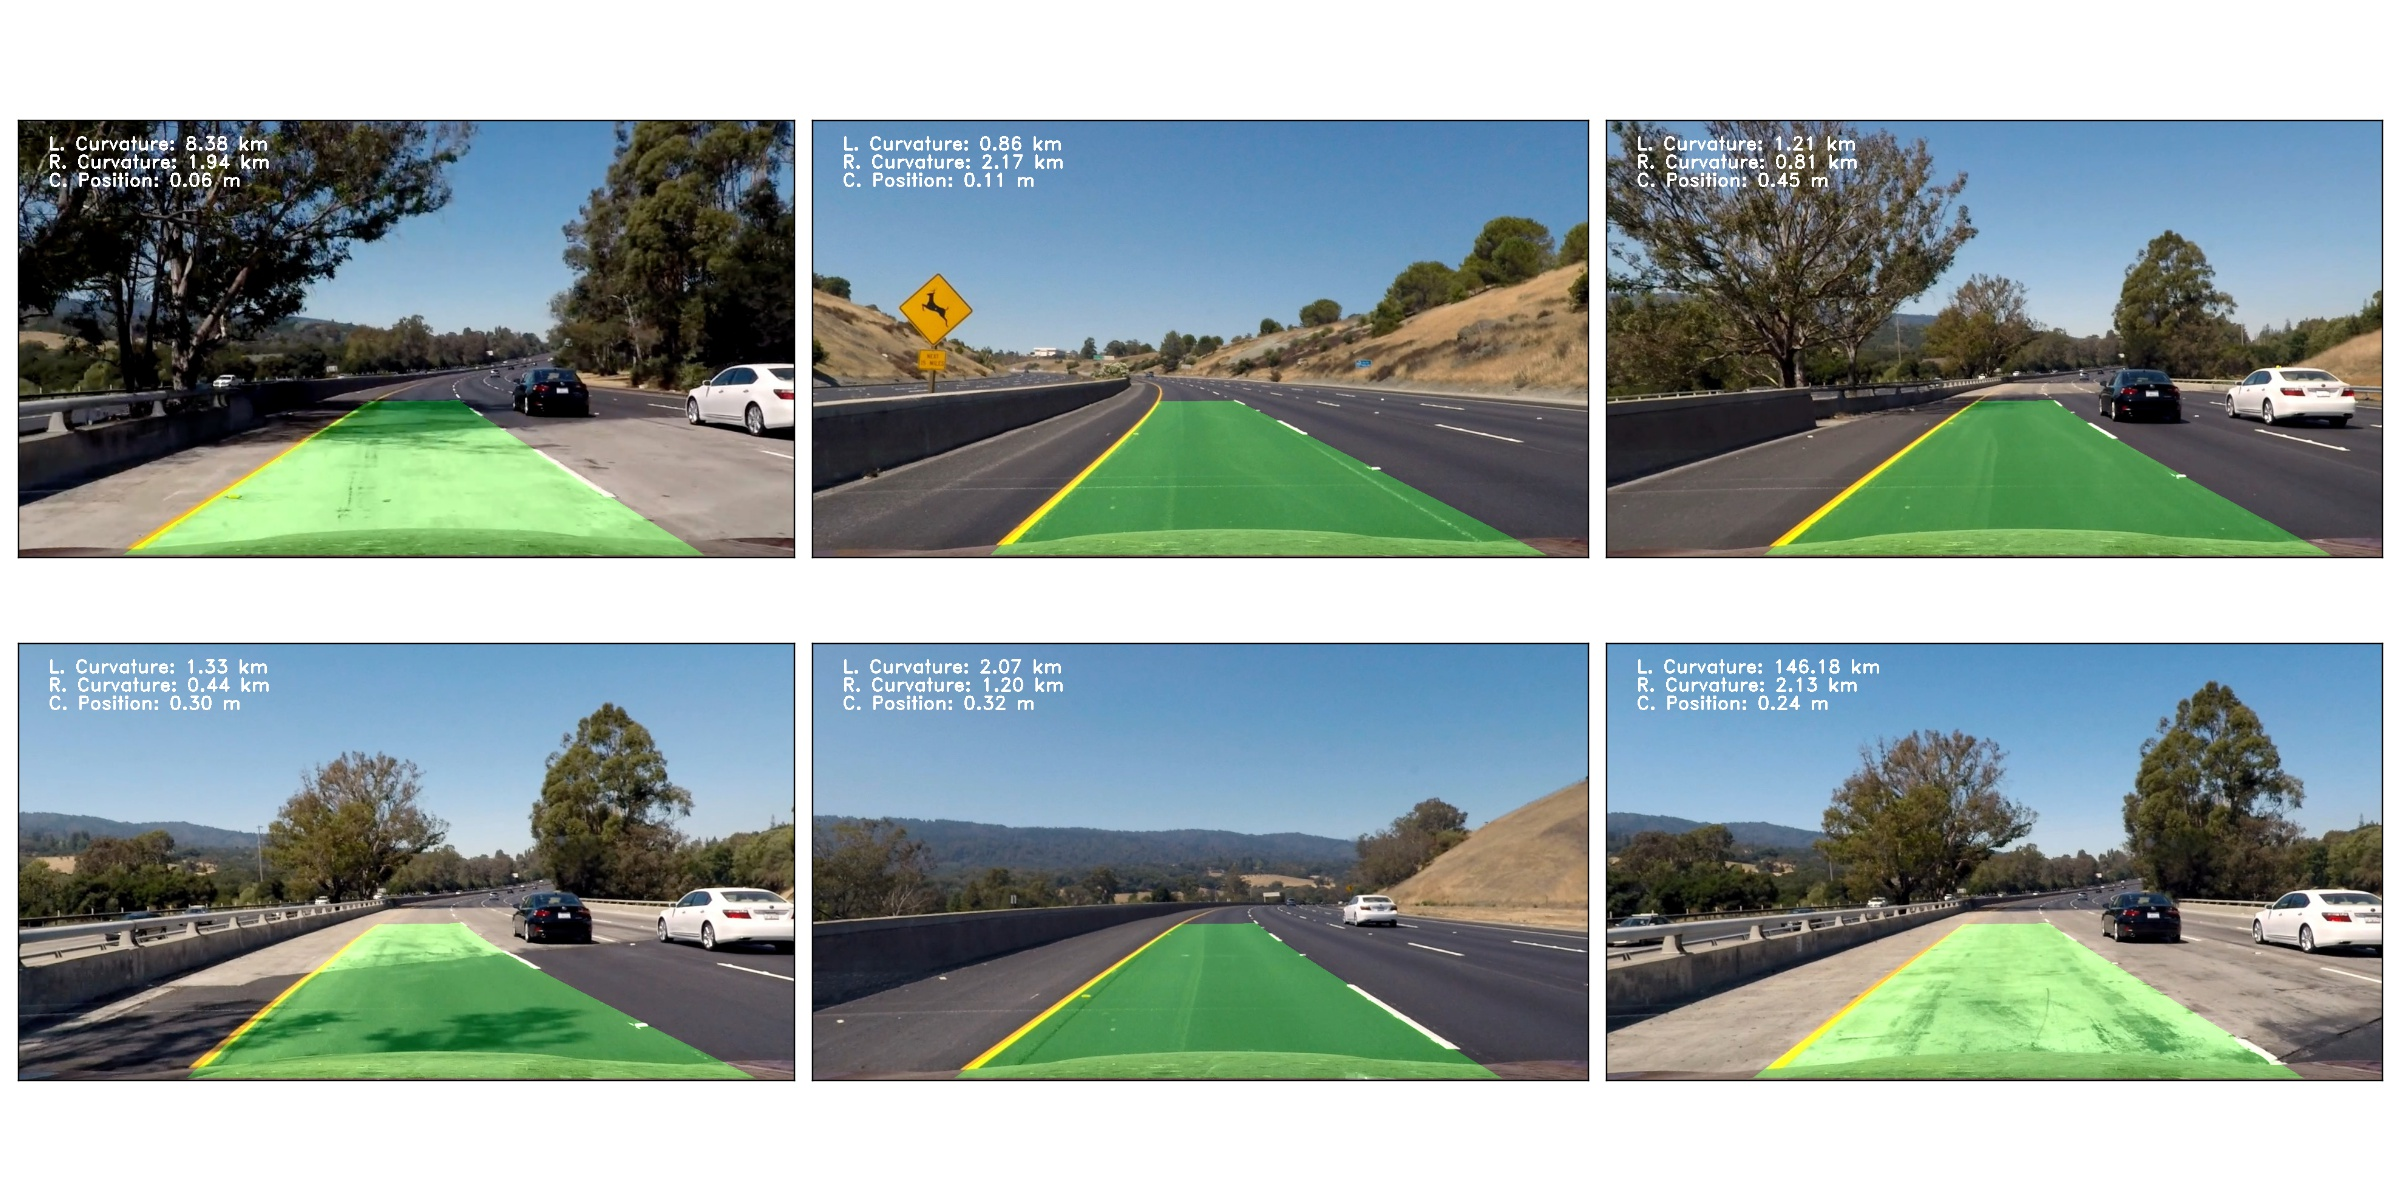
\includegraphics[width=.9\linewidth]{output_images/drawn_lanes_test_images.jpg}

Finally, generate a new processor and apply it to the video
stream.  We generate a new processor in order to give it a
different buffer size for the ring buffers supporting the
weighted averages.  For the video stream, the ring buffers have
50 slots, not 10.  Sinc ethe video stream is at 25 frames per
second, this constitutes a full 2 second window for the weighted
average.  That may seem like a lot, and we \emph{do} have to be
careful not to push it too far.  There is a trade-off between
the smoothness and robustness added by the weighted average, and
a stiffness to the model that may cause it to lag on sharp
turns.  In practice, however, the weighted average quickly
deweights older frames, and in experimentation no deleterious
effects were noticed with a set of 50-slot ring buffers.

\begin{verbatim}
in_clip = VideoFileClip("project_video.mp4")
out_clip = in_clip.fl_image(get_processor(50))
cProfile.run('out_clip.write_videofile("output_images/project_output.mp4", audio=False)', 'restats')
\end{verbatim}

We can see the result for the project video in the following
video clip.

\subsection*{Discussion}
\label{sec-2-3}

\subsubsection*{What Worked Well}
\label{sec-2-3-1}

\subsubsection*{What Could Be Improved}
\label{sec-2-3-2}
% <a href="http://www.gnu.org/software/emacs/">Emacs</a> 24.5.1 (<a href="http://orgmode.org">Org</a> mode 8.2.10)
\end{document}